\chapter{Enhancing Dynamic Maps for Multivariate Data}
\label{chap:MultivariateMaps}
\bibentry{mcnabb2019multivariateT} \cite{mcnabb2019multivariateT} \\
\chapterquote{A glyph representing multiple attributes may need simplifying when reduced in size, resulting in a loss of data.}
{Ellis and Dix, A taxonomy of clutter reduction for information visualisation \cite{ellis2007taxonomy}}



\newpage
{\footnotesize \hypersetup{linkcolor=black}
\minitoc}

%-------------------------------------------------------------------------
%\begin{abstract}
%\newpage
%\topskip0pt
%\vspace*{4cm}
%\section*{Chapter Abstract}
%Maps are one of the most conventional types of visualization used when conveying information to both inexperienced users and advanced analysts. However, the multivariate representation of data on maps is still considered an unsolved problem. We present a multivariate map that uses geo-space to guide the position of multivariate glyphs and enable users to interact with the map and glyphs, conveying meaningful data at different levels of detail. We develop an algorithm pipeline for this process and demonstrate how the user can adjust the level-of-detail of the resulting imagery. We present a selection of user options to facilitate the exploration process and provide case studies to support how the application can be used. We also compare our placement algorithm with previous geospatial glyph placement algorithms. The result is a novel glyph placement solution to support multi-variate maps.
%%\end{abstract}  
\clearpage
%-------------------------------------------------------------------------
\section{Introduction and Motivation} \label{sec:introMM}
In this chapter, we move toward extending our existing algorithm to support new features, including multivariate data and glyph placement. We also present the robustness of our design using real-time filters and animation.

Maps are useful for conveying information to both inexperienced and advanced users. There are many types of maps designed to present data but the underlying maps often come with other challenges such as how the areas are segmented. Fairbairn et al.\ suggest scale, level of detail, and multivariate data as common challenges for the representation of geo-spatial data \cite{fairbairn2001representation}.  Ward et al.\ state, \emph{``A problem of choropleth maps is that the most interesting values are often concentrated in densely populated areas with small and barely visible polygons, and less interesting values are spread out over sparsely populated areas with large and visually dominating polygons."} The challenge of perception (\textbf{C1} -- size perceivability) is a fundamental one associated with digital maps. Even when trying to rectify this for a univariate map, few solutions enable opportunities to convey multivariate, high-dimensional data. For example, geo-spatial designs (choropleths, cartograms, symbol maps, etc.) only depict uni-variate, or occasionally, bivariate data. This is a challenge for conveying of multi-variate geospatial data (\textbf{C2} -- multivariate geospatial data). One possibility is glyphs to support multivariate visualization options. However, even if we can present multivariate geospatial data using glyphs, we still run into challenges. If we plot glyphs in their geospatial context, then we risk overlap and over-plotting. In other words, if we place a multivariate glyph at the center of each unit area on a map, the glyphs will either overlap in many cases or be too small to perceive, especially in densely populated areas (see Figure \ref{fig:ccgs}) (\textbf{C3} -- occlusion). Ellis and Dix state \emph{``a glyph representing multiple attributes may need simplifying when reduced in size, resulting in a loss of data"} \cite{ellis2007taxonomy}, suggesting that reducing the size of a scalable multivariate glyph can be problematic (\textbf{C1} -- size perceivability). Another option to address \textbf{\textbf{C3} -- occlusion} is to employ structure-driven glyph placement guided by a Cartesian grid. However, this common solution de-couples the glyphs from the original geospatial areas they intend to represent. This is the challenge of geo-spatial glyph-placement (\textbf{C4} -- glyph placement).
In order to address all four challenges, \textbf{C1--C4}, we introduce scale-aware maps, a process of presenting geospatial multivariate data based on the desired screen space,  that enables dynamic modification to the level of detail shown using both zooming functions and custom scale options. We integrate this with glyphs to present multivariate data in a geospatial context to enable interactive exploration and facilitate easier comprehension with area context using both smooth transitions and uncertainty indicators. We refer to our work as using glyphs as opposed to symbols guided by the definition from Borgo et al.\ who define a glyph as, \emph{``...an independent visual object that depicts attributes of a data record"} \cite{borgo2013glyph}. Our contributions include:
\begin{figure*}[t]
\centering
%\subfigure[]{
%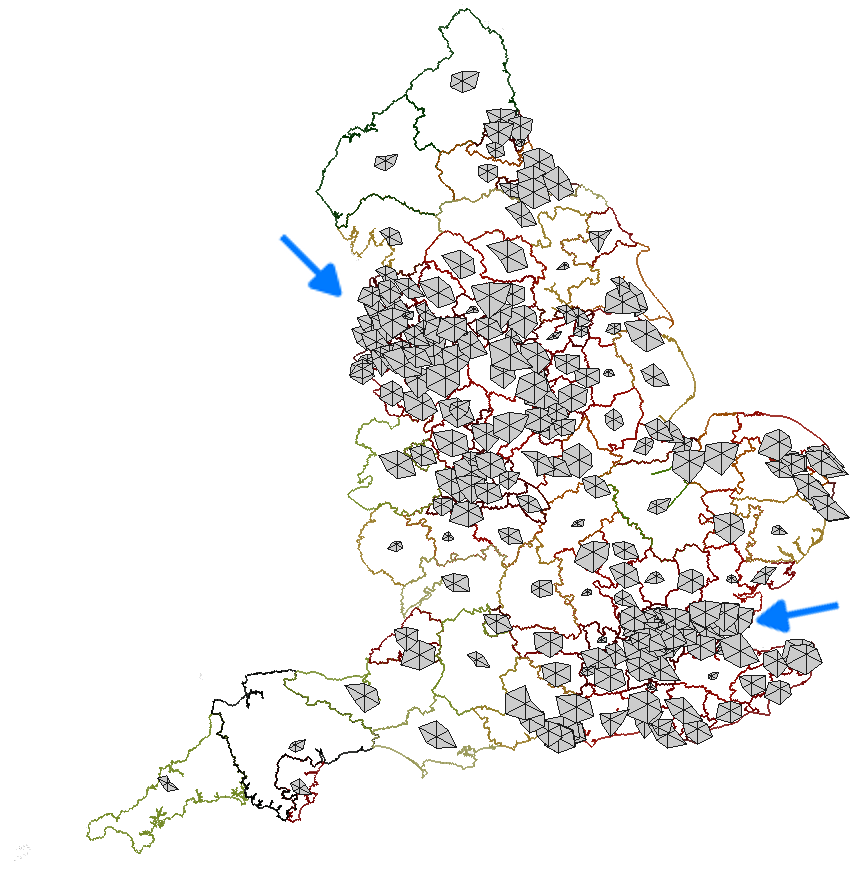
\includegraphics[width=0.4\textwidth]{images/CCGStarDefault.png}}
%\subfigure[]{
%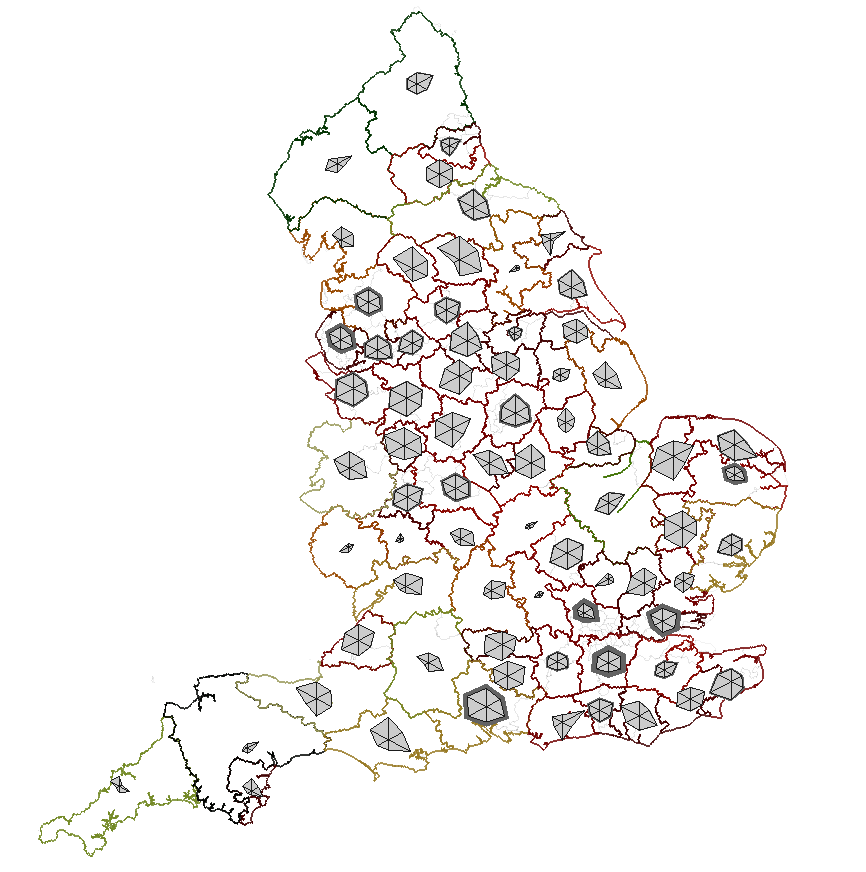
\includegraphics[width=0.4\textwidth]{images/CCGStarBasic.png}}
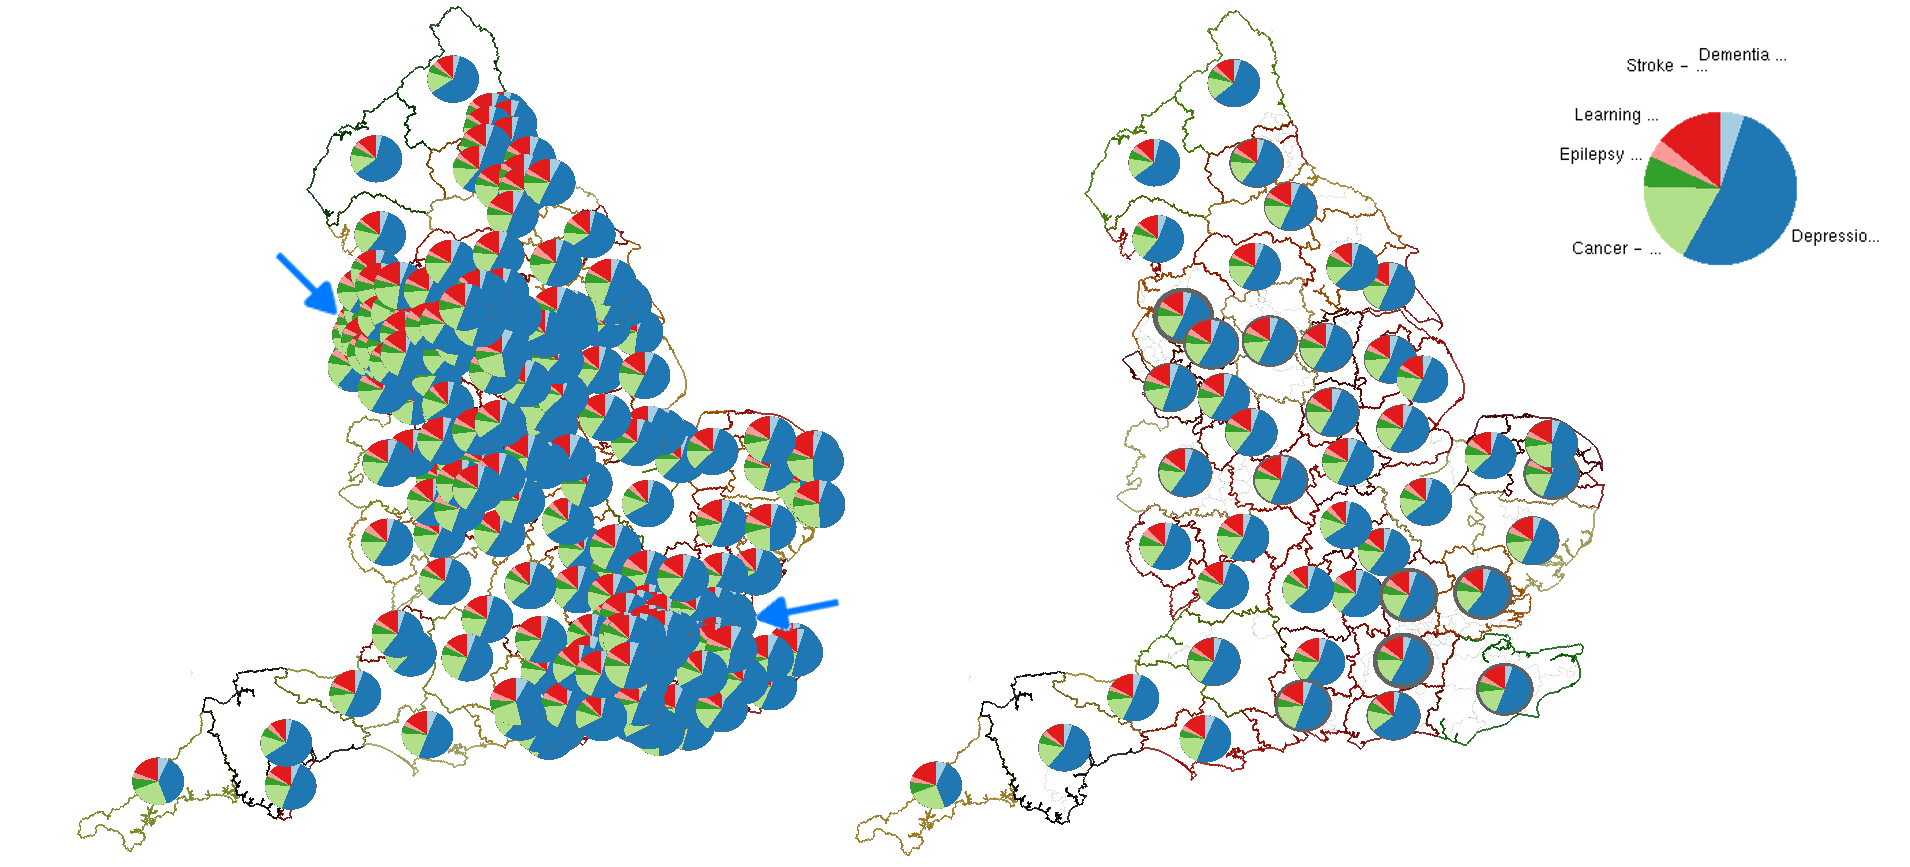
\includegraphics[width=0.95\textwidth]{images/ch5/ccgsetPie2}
\caption{(left) The representation of population health data based on the Clinical Commissioning Groups (CCGs) of England \cite{publicHealthEngland}. Refer to Section \ref{sec:case} for a case study. Glyphs that are simply placed at the centroid of each region are over-plotted and occluded around London, Manchester, and Liverpool (indicated by blue arrows). (right) Our result using level-of-detail scale-aware maps. Even at a small scale for the figure, we can still clearly differentiate each area's glyph.} \label{fig:ccgs}
\end{figure*}


\noindent\textbf{1.} A multivariate map with scalable glyph rendering and presentation (in the form of scale-aware maps) (\textbf{C1} -- size perceivability, \textbf{C2} -- multivariate geospatial data, \textbf{C4} -- glyph placement).\\
\textbf{2.} Dynamic hierarchical glyphs that support zooming, and user-controlled level of detail. (\textbf{C2} -- multivariate geospatial data, \textbf{C3} -- occlusion, \textbf{C4} -- glyph placement)\\
\textbf{3.} Interactive filters to improve analysis and exploration of multivariate data and comparison of geo-spatial areas. (\textbf{C2} -- multivariate geospatial data)\\
%\end{itemize}
In order to do so, we develop solutions that address the four major challenges, \textbf{C1--C4}.

%-------------------------------------------------------------------------

\section{Background}
Our literature review in Chapter \ref{chap:SoS} includes a section of glyph-focused survey papers, as well as geospatial surveys.  Borgo et al.\ present a survey of glyph design criteria \cite{borgo2013glyph}. Fuchs et al.\ provide a systematic review of experimental studies on data glyphs \cite{fuchs2016systematic}.
Ward presents a taxonomy of different glyph placement strategies (discussed further in the glyph placement section) \cite{ward2002taxonomy}. We find three survey papers on cartograms \cite{tobler2004thirty, nusrat2015task, nusrat2016state}. We do not consider univariate cartograms within the scope of our work as they distort the boundary geometry of the geospatial data, which we avoid in our process. We do not consider magic lenses in our related work \cite{tominski2014survey}. We make this decision considering that magic lenses are manually manipulated, are typically not coupled to geospace, do not necessitate a placement algorithm, and their border transitions are not necessarily smooth \cite{tominski2016interactive}. Although we discuss focus+context in the paper, we focus our related work on the topic of maps and glyph placement. We recommend Cockburn et al.\ for discussion on the topic \cite{cockburn2008review}. 
Bekos et al.\ present a taxonomy on label placement techniques \cite{bekos2019external}. We do not consider labels as related work as they do not necessarily apply to multivariate data, and labels do not have to follow a cohesive hierarchical structure \cite{luboschik2008particle}. However the work here could likely be adapted specifically for labeled maps. 

\textbf{ Aggregation Techniques:~}
Janicke et al.\ use a circle packing method to reduce the complexity of point-based data at multiple levels of detail \cite{janicke2012comparative}. The user can zoom in and out of the map while the point distribution is aggregated to present clear, visible point frequencies. This differs from our work as the data is not coupled to geospatial areas. We also focus on multivariate data which is not featured in their work.
Rohrdantz et al.\ present a multivariate map depicting different new trends across the world using the geospatial map and data proportional glyphs\ \cite{rohrdantz2012s}. They use geo-tagging to aggregate their data and do not present any techniques to avoid occlusion. This differs from our work which aims to present glyphs as concisely as possible and handles multiple levels of detail with dynamic zooming. 
Jo et al.\ present a model for reducing complexity in presenting multiclass data on maps by using aggregative techniques \cite{jo2019declarative}. Their work emphasizes techniques to increase perceivability without manipulating the underlying geospatial context, whilst ours focuses on increasing perceivability of existing techniques through geospatial unification.
Guo creates a technique known as regionalization with dynamically constrained agglomerative clustering and partitioning (REDCAP) \cite{guo2008regionalization}. Rather than focus on scale, the algorithm focuses on agglomerating clusters and discusses six variations of their methodology. Although their technique can calculate the varying number of regions, they do not discuss how the number of regions are selected, which differs from our work that dynamically allows restructuring of the hierarchy. The method uses region-based plotting, does not use glyphs, does not consider multivariate data, nor support dynamic zooming.

\textbf{Cartograms:~}
Dorling visualizes local urban changes across Great Britain \cite{dorling1995visualization}. The paper uses multivariate options to review industry distribution, owner-occupied housing, as well as a set of attributes plotted using Chernoff faces as an equal area representation.
Slingsby et al.\ capture the geo-spatial context and transform their results into a grid, which is then represented by a treemap where the hierarchy is based on temporal data \cite{slingsby2010treemap}.
 Slingsby et al.\ present a rectangular cartogram showing the postcodes in Great Britain, where postcode district and unit postcodes form the hierarchy \cite{slingsby2010rectangular}. Cartograms distort geo-space, which we avoid using our procedure.
Tong et al.\ develop Cartographic Treemaps to explore multivariate medical data provided by Public Health England \cite{tong2017cartographic}. This is extended to time-varying data \cite{tong2017time}. 
Beecham et al.\ visualize trends to explain the UK's vote to leave the European Union  \cite{beecham2018locally}. They use a juxtaposed view to presented equal area cartograms for different variants. 
Nusrat et al.\ produce a cartogram that presents bi-variate data using a ring encoding, where the color presents the leading statistic, and the ring thickness presents the value the leading statistic leads by \cite{nusrat2018cartogram}. This differs from our work by emphasizing bivariate design, whilst we provide options for up to nine dimensions to be represented clearly. Our method also supports interactive levels of detail with dynamic zooming.

\textbf{Multivariate Maps:~} Multivariate maps have been used in cartography for over 100 years. For example, Minard depicts a multivariate map using pie charts to present cow consumption across France \cite{minard1858carte}. The pie charts are placed manually.
Kahrl et al.\ present a range of imagery focused on California's water supplies including irrigation applied to crops in the form of dense pixel displays across geospatial points \cite{kahrl1978california}. 
Approaches to add more dimensions to choropleths include bivariate color maps \cite{olson1981spectrally, dunn1989dynamic}.
Brewer and Campbell present point symbols for representing quantitative data on maps, including bi-variate options \cite{brewer1998beyond}. Although their paper does not focus on glyph placement, their examples place symbols on a region's centroid and exhibit minor occlusion.
Andrienko and Andrienko \cite{andrienko2006exploratory} contains a range of examples of multivariate maps using glyphs for thematic maps, including temporal glyphs, and multivariate pie glyphs for forest data. They present glyph placement two ways: region-centroid symbol placement for US states and a Cartesian grid to represent forest data over Europe \cite{andrienko2006exploratory}. They discuss the importance of the link between identifying a symbol and the geo-space it represents (on the map) (\textbf{C4} -- glyph placement).
Slocum et al.\ provide a chapter on multivariate maps, describing techniques to consider when displaying bivariate, trivariate, and multivariate data \cite{slocum2009thematic}. 
Bertin's Semiology of Graphics is a foundational work on cartography. The work covers many different maps including multivariate maps of up to 6 variates, using grid-based and coordinate-based placement schemes \cite{bertin1983semiology}.
Elmer review symbol consideration for bivariate thematic maps, but do not support more than two variates \cite{elmer2012symbol}. Our algorithm supports an arbitrary number of variants depending on the glyph design.
Kresse and Danko present geographic techniques from basic principles to applications \cite{kresse2012springer}. They present a table of visual variables to represent data, applied to a given map and symbols.
Tsorlini et al.\ present a taxonomy of thematic cartography symbols, including multivariate options \cite{tsorlini2017designing}. The symbols are presented as a hierarchy, focusing on the number of attributes, and arrangement. The focus on this work is not on glyph placement, nor dynamic level-of-detail.


\textbf{General Glyph Placement:~} 
This section encompasses the rest of the work on glyph placement not connected to other background groups. Ward and Lipchak create a software tool for cyclical, temporal multivariate data. Glyphs are placed in an ordered grid structure to enable easy comparison between similar months, or entire years \cite{ward2000visualization}. They also use a radial structure. Our work differs from this work by focusing on the glyph placement coupled to geospatial areas. 
Ward presents a taxonomy of different glyph placement strategies \cite{ward2002taxonomy}. They introduce glyph designs that can be used, and 15 glyph placement strategies together with a flow chart of how the glyph placement is driven (data-driven or structure-driven). Our placement strategy is considered geo-spatially data-driven. As the modifications are made before the placement process, it falls into original\arrow{}derived\arrow{}data-driven. This is expanded by a subsection in a further survey by Ward \cite{ward2008multivariate}.
Ropinski and Preim present a taxonomy of usage guidelines for glyph-based medical visualization \cite{ropinski2008taxonomy}. As opposed to Ward's placement taxonomy, they suggest glyphs should be placed based on physical characteristics or anatomical features.
Borgo et al.\ provide a section on glyph placement which extends on both of the previous taxonomies by suggesting user-driven placement \cite{borgo2013glyph}.
Chung et al.\ discuss glyph sorting strategies and present horizontal axis bins, applying them to sport-event analysis glyphs \cite{chung2015glyph}. Our work differs by guiding our glyph placement strategy based on a 2D geospatial context. As evidenced by Table \ref{tbl:related}, the algorithm we present offers a novel combination of glyph placement, multivariate data, level of detail, dynamic zooming, and smooth transitions.

\begin{table*}[t]\centering \scriptsize
%\rowcolors{1}{white}{black!05}
\begin{tabularx}{1\linewidth}{|c|c|C|C|C|C|C|}\hline \rowcolor{black!15}
\multicolumn{2}{|c|}{\textbf{Literature}}&\textbf{Placement Algorithm}&\textbf{Max No. of Variates}& \textbf{Level-of-Detail}&\textbf{Dynamic Zooming}&\textbf{Smooth Transitions}\\ \hline
\rowcolor{black!05}\header&\header Janicke et al.\ \cite{janicke2012comparative} & Coordinate-based & \color{red} 1 & \cmark & \cmark & \xmark \\ \specialRule
\header &\header Rohrdantz et al.\ \cite{rohrdantz2012s} & Coordinate-based & \greenfont 5 & \xmark & \xmark & \xmark \\ \specialRule
\rowcolor{black!05}\header&\header Jo et al.\  \cite{jo2019declarative} & Region centroid & \greenfont 10 & \xmark & \xmark & \xmark \\ \specialRule
\header \multirow{-4}{*}{\rotatebox{90}{\fontsize{7}{7}\textbf{Aggregation}}} & \header Guo \cite{guo2008regionalization} & No glyphs & \color{red} 1 & \cmark & \xmark & \xmark \\ \hline

\header &\header Minard \cite{minard1858carte}& Manual & \greenfont 3 & \xmark & \xmark & \xmark \\ \specialRule
\rowcolor{black!05}\header&\header Kahrl et al.\ \cite{kahrl1978california} & Manual &\greenfont 6&\xmark&\xmark&\xmark \\ \specialRule
\header&\header Olson \cite{olson1981spectrally}& No glyphs & 2&\xmark&\xmark&\xmark \\ \specialRule
\rowcolor{black!05}\header&\header Dunn \cite{dunn1989dynamic}& No glyphs & 2&\xmark&\xmark&\xmark \\ \specialRule
\rowcolor{black!05}\header&\header Brewer \cite{brewer1998beyond}&Region centroid&2&\xmark&\xmark&\xmark \\ \specialRule
\header&\header Andrienko and Andrienko \cite{andrienko2006exploratory}&Region centroid/ Grid-based&\greenfont 6&\xmark&\xmark&\xmark \\ \specialRule
\rowcolor{black!05}\header&\header Slocum et al.\ \cite{slocum2009thematic}&Region centroid/ Grid-based&\greenfont 8&\xmark&\xmark&\xmark \\ \specialRule
\rowcolor{black!05}\header&\header Bertin \cite{bertin1983semiology}&Coordinate-based/ Grid-based&\greenfont 6&\xmark&\xmark&\xmark \\ \specialRule
\header&\header Elmer \cite{elmer2012symbol}&Region centroid& 2&\xmark&\xmark&\xmark \\ \specialRule
\rowcolor{black!05}\header&\header Kresse and Danko \cite{kresse2012springer}&Coordinate-based& 2&\xmark&\xmark&\xmark \\ \specialRule
\rowcolor{black!05}\header\multirow{-14}{*}{\rotatebox{90}{\textbf{Multivariate Maps}}}&\header Tsorlini et al.\ \cite{tsorlini2017designing}&Region centroid&\greenfont 6&\xmark&\xmark&\xmark \\ \hline

%\header&\header Dorling \cite{dorling1995visualization}&Cartographic Layout&\greenfont 8&\xmark&\xmark&\xmark \\ \specialRule
%\header&\header Slingsby et al.\ \cite{slingsby2010treemap}&No Glyphs&\color{red} 1&\xmark&\xmark&\xmark \\ \specialRule
%\rowcolor{black!05}\header&\header Slingsby et al.\ \cite{slingsby2010rectangular}&No Glyphs&\color{red} 1&\xmark&\xmark&\xmark \\ \specialRule
%\header&\header Tong et al.\ \cite{tong2017cartographic,tong2017time}&No Glyphs&\greenfont 14&\xmark&\xmark&\xmark \\ \specialRule
%\header&\header Beecham et al.\ \cite{beecham2018locally}&No Glyphs&\greenfont 6&\xmark&\xmark&\xmark \\ \specialRule
%\rowcolor{black!05}\header\multirow{-6}{*}{\rotatebox{90}{\textbf{Cartograms}}}&\header Nusrat et al.\ \cite{nusrat2018cartogram}&Cartographic layout& 2&\xmark&\xmark&\xmark \\ \hline


\header \textbf{GGP} &\header Chung et al.\  \cite{chung2015glyph}&Scatterplot&\greenfont 9&\xmark&\xmark&\xmark \\ \hline \hline



\header&\header McNabb et al.\ \cite{mcnabb2018dynamic} & No glyphs & \color{red} 1 & \cmark & \cmark & \xmark \\ \hline
\rowcolor{black!05}\header&\header \textbf{This} & \textbf{Dynamic Region centroid} &\greenfont \textbf{9} & \textbf{\cmark} & \textbf{\cmark} & \textbf{\cmark} \\ \hline

\end{tabularx}
\caption{A breakdown of the related literature. For each paper, we review the type of placement algorithm used, the number of data variates presented, if multiple levels-of-detail are depicted of the data, whether dynamically moving between levels of detail is discussed, and if so, whether smooth transitions are implemented to increase recognition of dynamic glyphs. The table is sorted into aggregation, multivariate maps, and general glyph placement (GPP) literature. \vspace{-0.2cm}} \label{tbl:related}
\end{table*}

\begin{figure*}[t]
\centering
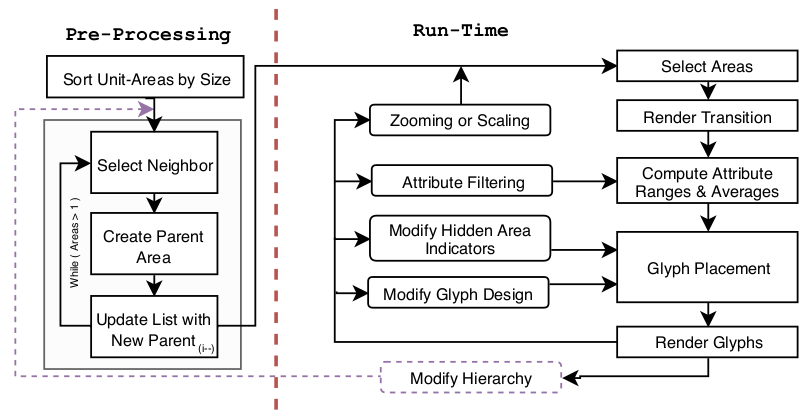
\includegraphics[width=0.6\textwidth]{images/ch5/HorizontalFlowv4}\vspace{-0.3cm}
\caption{The flow chart of the procedure. The right dashed, red line represents what is discussed in the scope of this paper. The pre-processing steps are discussed by McNabb et al.\ in detail \cite{mcnabb2018dynamic}. See Section \ref{fig:overview} for a complete description of the run-time procedure.} \label{fig:procedure}
\end{figure*}
\section{Design Goals and Tasks} \label{sec:tasks}
We derive six mains tasks to motivate our design process. \\
\textbf{T1}\textbf{ -- Overview:} Provide a glyph-based overview of multivariate data on a map free from occlusion (\textbf{C3} -- occlusion).\\
\textbf{T2}\textbf{ -- Multivariate Map:} Offer a selection of informative multivariate glyphs to compare trends between regions (\textbf{C2} -- multivariate geospatial data).\\
\textbf{T3}\textbf{ -- Glyph Placement:} Clearly couple encoded glyphs to their geo-spatial contexts (\textbf{C4} -- glyph placement).\\
\textbf{T4}\textbf{ -- Level-of-detail} Leverage scale-aware maps to enable exploration of the data at multiple levels of detail (\textbf{C1} -- size perceivability).\\
\textbf{T5}\textbf{ -- Filtering:} Support the exploration of multivariate geo-spatial data with user options with varying glyph designs and filters (\textbf{C2} -- multivariate geospatial data).\\
\textbf{T6}\textbf{ -- Smooth Interaction:} To provide smooth and fluid transitions between the different levels of detail (\textbf{C4} -- glyph placement).
\section{Overview} \label{fig:overview}
This section provides the pre-processing steps used to create the scale-aware maps, the run-time process for transitioning between glyph densities, and the options we provide to enhance the exploration of the data. The pre-processing steps are based on  previous work by McNabb et al \cite{mcnabb2018dynamic}. The purpose of the pre-processing step is to build a map whose areas are always perceivable, unit areas that are too small \cite{mcnabb2018when} are unified until they reach a minimum area threshold set by the user. The area-based hierarchy construction is a recursive algorithm broken down into three sub-routines. In these three steps, we select the optimal neighbor for merging, we identify the shared boundary between the given area and its neighbor, and unify them to create a new area which is then inserted back into the list of areas sorted by size. A flow chart of the procedure is found in Figure \ref{fig:procedure}. 
Once the pre-processing steps are completed, we move to our run-time implementation. The first step is to identify optimally-sized areas, render any transitions between previously rendered and the newly selected areas, compute the glyph visual mapping of the data, and update the glyph properties, before rendering the glyphs. From here, we provide five options to transform the view. Zooming or scaling to dynamically modify the multi-variate glyphs, attribute filtering to modify the glyph properties and mapping, modification of hidden area indicators to customize glyph design, the revision of glyph attributes to customize the glyph design, and modification of the underlying hierarchy which returns the algorithm to the pre-processing procedures. We discuss the steps in detail in the sections that follow.

\subsection{Pre-processing}
%\textbf{Order Vertices:}
%\textbf{Order Vertices:}
We use a recursive procedure to create a hierarchical area-based data structure. An area hierarchy is created for each contiguous region, where each area is merged with its closest neighbor identified using a customizable distance metric \cite{mcnabb2018dynamic}. We start with a merge candidate list filled with the sorted unit-areas (for one contiguous region). There are three main sub-routines: (a) neighbor selection, (b) creating the parent area, and (c) updating the merge candidate list. If only a single unit-area remains in the merge candidate list, no further merges can be processed and the procedure terminates. (a) In order to select an appropriate neighbor to join, we use a general and flexible distance metric for amalgamation evaluated between neighboring areas.

We use the closest distance considered as the optimal selection for a neighbor,
$D = w_a.\frac{a}{a_{max}} + w_d.\frac{d}{d_{max}} + w_\alpha.\frac{\alpha}{\alpha_{max}} + w_{b_s}.(1-\frac{b_s}{b_{s_{max}}})$.
The measure consists of four constituents: Smallest area ($a$), euclidean distance between centroids ($d$), univariate data value variance ($\alpha$), and shared boundary resolution ($b_s$). We search and identify each common vertex between neighboring areas to identify the shared boundary. We update the sorted area list by removing the two merged areas and inserting the newly created parent, which may be used as a new merge candidate. This is repeated until only one area remains in each contiguous region.\\
\textbf{Value calculation for unified areas:} The Modifiable Areal Unit Problem (MAUP) \cite{openshaw1984modifiable} is an important aspect to consider when discussing the modification of boundaries or values. We address this by providing the user options to customize the calculation of aggregated univariate data values as well as the customizable distance metric used to evaluate area merge candidates. The data is linked to the unit areas during the initial loading of the shapefiles. Before the area tree is built, the user can select the type of value amalgamation. This enables the user to choose options of sums,  frequencies, and value averages. When amalgamating values using sums, the value can be calculated using aggregation. Qualitative values are calculated using frequencies. For a detailed description of parent value calculation, see Chapter \ref{chap:dcm}.
\subsection{Geospatial Glyph Placement} \label{sec:rendering}
In order to enable multi-variate maps, a number of technical challenges must be addressed including: 1) A glyph-placement strategy, 2) A hierarchical glyph design, 3) dynamic level-of-detail support, 4) smooth transitions between child and parent glyphs, 5) multi-variate filtering and selection, and 6) customizable interactive user options. Furthermore, the hierarchical glyph design must support the encoding of aggregation error.

We select visible areas and glyphs based on a minimum area scale requirement (a percentage), $m$ (see Section \ref{sec:scaleAdjust}). When the map is rendered, the tree is traversed using a depth-first search (DFS) to identify which areas are rendered. If an area is larger than $m$ we test two criterion: if the area is a leaf node, or if either the left or right child is smaller than $m$. If either of these are true, we render the area. For each area displayed, we create a glyph using the area's centroid to position the glyph. We create a glyph that reflects the given area's multivariate data values (based on the user's selection, see Section \ref{sec:glyphSelect}). We first set the size of the glyph at 2.5\% of the screen space as the default, a heuristic we derive from McNabb et al.'s previous user study on perception of scale on choropleth maps \cite{mcnabb2018when}. As the zoom level of the map changes, different areas may meet $m$ and therefore be presented, creating a dynamic presentation of glyphs. This addresses \textbf{T1 -- Overview} and \textbf{T3 -- Glyph Placement}, by providing a clear overview of the map with no occlusion, and clearly encoded geospatial context. As the size of the glyph changes so does the perceived ideal map structure. The user can manually find their own perceived preference using sliders or using naive estimated glyph placement (see Section \ref{sec:options}).

\begin{figure*}[h]
\centering
%\subfigure{
%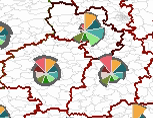
\includegraphics[width=0.18\linewidth]{images/transition/01.png}}
%\subfigure{
%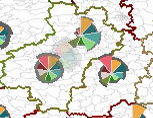
\includegraphics[width=0.18\linewidth]{images/transition/02.png}}
%\subfigure{
%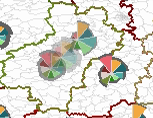
\includegraphics[width=0.18\linewidth]{images/transition/03.png}}
%\subfigure{
%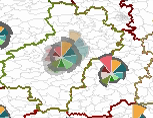
\includegraphics[width=0.18\linewidth]{images/transition/04.png}}
%\subfigure{
%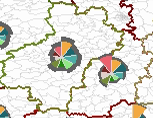
\includegraphics[width=0.18\linewidth]{images/transition/05.png}}
\subfloat{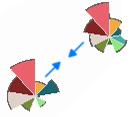
\includegraphics[width=0.12\linewidth]{images/ch5/transition/11}}
\subfloat{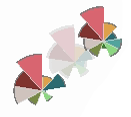
\includegraphics[width=0.12\linewidth]{images/ch5/transition/12}}
\subfloat{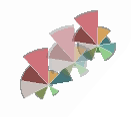
\includegraphics[width=0.12\linewidth]{images/ch5/transition/13}}
\subfloat{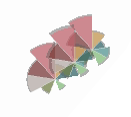
\includegraphics[width=0.12\linewidth]{images/ch5/transition/14}}
\subfloat{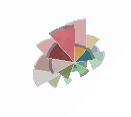
\includegraphics[width=0.12\linewidth]{images/ch5/transition/15}}
\subfloat{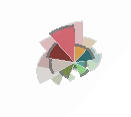
\includegraphics[width=0.12\linewidth]{images/ch5/transition/16}}
\subfloat{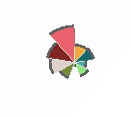
\includegraphics[width=0.12\linewidth]{images/transition/17}} \vspace{-0.5cm}
\caption{An example of a smooth transition made between two child glyphs that translate toward the new parent node. Both child glyphs decrease in opacity, whilst the new parent glyph increases in opacity. Refer to Section \ref{sec:transitions}. See also the accompanying video for this dynamic behavior (Section \ref{sec:video}).}  \label{fig:transitions}
\end{figure*}

\begin{figure}[ht!]
\centering
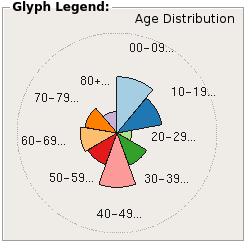
\includegraphics[width=0.4\textwidth]{images/GlyphLegend2} 
\caption{A representation of a glyph legend. The data represents the prevalence of population per age range. The dotted circle represents the full scale of the glyph or the largest value for each dimension. The glyph legend shows the average values over the whole data set. Refer to Section \ref{sec:legend}.} \label{fig:legend}
\vspace{-0.2cm}
\end{figure}

\begin{table*}[t] \centering
\begin{tabular}{|m{2.5cm}|m{2.0cm}|m{2.0cm}|m{2.0cm}|m{2.0cm}| >{\centering\arraybackslash}m{2.4cm}|} \hline
&\multicolumn{5}{c|}{Hidden Density Indicators}\\ \cline{2-6}
\multirow{-2}{2.5cm}{\centering Glyph Design}&\centering No Indicator &\centering Outline &\centering Size &\centering Shadow & Size + Outline\\ \hline &&&&& \vspace{-1cm}\\ 
\centering Pie Chart&
\Centerstack{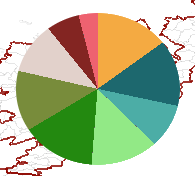
\includegraphics[width=\linewidth]{images/ch5/glyphs/2/pie0.png}}&
\Centerstack{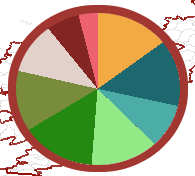
\includegraphics[width=\linewidth]{images/ch5/glyphs/2/pie1.png}}&
\Centerstack{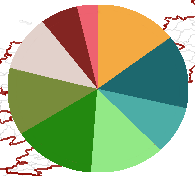
\includegraphics[width=\linewidth]{images/ch5/glyphs/2/pie2.png}}&
\Centerstack{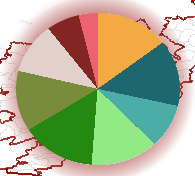
\includegraphics[width=\linewidth]{images/ch5/glyphs/2/pie3.png}}&
\Centerstack{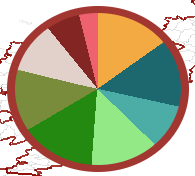
\includegraphics[width=0.9\linewidth]{images/ch5/glyphs/2/pie4.png}}\\
\centering Polar Area Chart&
\Centerstack{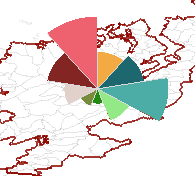
\includegraphics[width=\linewidth]{images/ch5/glyphs/2/wheel0.png}}&
\Centerstack{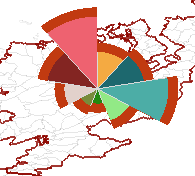
\includegraphics[width=\linewidth]{images/ch5/glyphs/2/wheel1.png}}&
\Centerstack{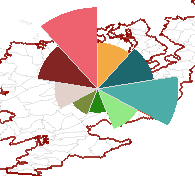
\includegraphics[width=\linewidth]{images/ch5/glyphs/2/wheel2.png}}&
\Centerstack{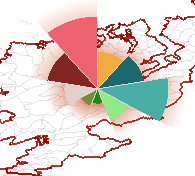
\includegraphics[width=\linewidth]{images/ch5/glyphs/2/wheel3.png}}&
\Centerstack{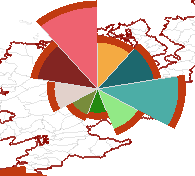
\includegraphics[width=0.9\linewidth]{images/ch5/glyphs/2/wheel4.png}}\\
\centering Bar Chart&
\Centerstack{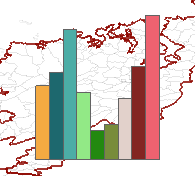
\includegraphics[width=\linewidth]{images/ch5/glyphs/2/bar0.png}}&
\Centerstack{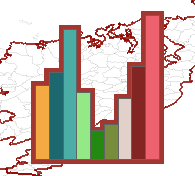
\includegraphics[width=\linewidth]{images/ch5/glyphs/2/bar1.png}}&
\Centerstack{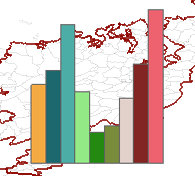
\includegraphics[width=\linewidth]{images/ch5/glyphs/2/bar2.png}}&
\Centerstack{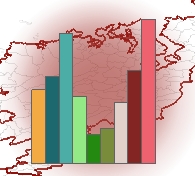
\includegraphics[width=\linewidth]{images/ch5/glyphs/2/bar3.png}}&
\Centerstack{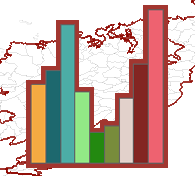
\includegraphics[width=0.9\linewidth]{images/ch5/glyphs/2/bar4.png}}\\
\centering Star Chart&
\Centerstack{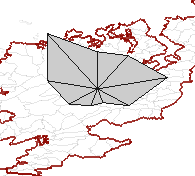
\includegraphics[width=\linewidth]{images/ch5/glyphs/2/star0.png}}&
\Centerstack{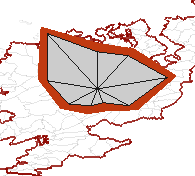
\includegraphics[width=\linewidth]{images/ch5/glyphs/2/star1.png}}&
\Centerstack{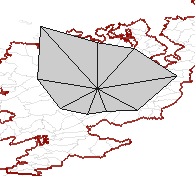
\includegraphics[width=\linewidth]{images/ch5/glyphs/2/star2.png}}&
\Centerstack{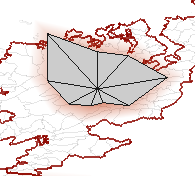
\includegraphics[width=\linewidth]{images/ch5/glyphs/2/star3.png}}&
\Centerstack{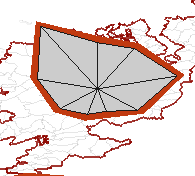
\includegraphics[width=0.9\linewidth]{images/ch5/glyphs/2/star4.png}}\\
\hline
\end{tabular}%\vspace{-0.3cm}
\caption{ Previews of the different glyphs, and the hidden density indicators provided in the application. Each glyph represents the same area, reflecting the same hidden indicator values, and attributes. Refer to our third case study, Section \ref{sec:case}, for more details on the values.} \label{tab:glyph}
\end{table*}

\subsection{Glyph Selection} \label{sec:glyphSelect}
We provide the user with four common glyph design options to represent the data (see Table \ref{tab:glyph}). We chose these four typical options due to their common occurrence in geospatial literature \cite{andrienko2006exploratory}. However, the principles we describe can be applied to any multi-dimensional glyph. The user can switch between each glyph design at any point once the hierarchical data structure has been built. These glyph options are:\\
\textbf{Pie Chart:} Pie charts are an easily recognizable and practical design, making it a suitable option to present multivariate data. Pie charts are primarily used to present distribution per geospatial area, where the angle of a segment is mapped to each data dimension proportionally. See Table \ref{tab:glyph}.\\
\textbf{Polar Area Chart:} Originally published by Nightingale \cite{nightingale1858notes}, a polar area chart is another radial plot but with equal segment angles. The radius or each slice corresponds to the values of each dimension, which facilitates comparison between geospatial areas. The polar area chart features different names including the wheel, coxcomb, or wing chart. See Table \ref{tab:glyph}. \\
\textbf{Bar Chart:} The bar chart is one of the most visually recognizable visual designs. Values are assigned to bar heights. aligned to the horizontal axis for easy value comparison. See Table \ref{tab:glyph}.\\
\textbf{Star Glyph:} Originally presented by Siegel et al.\cite{siegel1972surgical}, a star glyph presents values using lines originating from the same point, at equal angles. The endpoints connect to form a unique polygon based on the length of each line. See Table \ref{tab:glyph}.\\ This addresses the requirements for \textbf{T2 --Multivariate Maps}. We choose four standard glyph designs as a proof-of-concept. Glyph placement, not glyph design is the focus of this paper. The principles we present can be extended to any multivariate glyph.

\subsection{Adjusting Level-of-Detail with Glyph Density} \label{sec:scaleAdjust}
Adjusting glyph density can be handled in two different ways. First, we give the user a slider which depicts $m$, a minimum area requirement. The parameter $m$ represents a percentage of screen space. This is used as the primary variable for the depth-first search (DFS) discussed in Section \ref{sec:rendering}. We also allow the user to interactively zoom in or out of the map. This changes the visible extents of the map, modifying the screen space covered by each area. These options enable the rendering of perceivable glyphs, meeting the requirements for \textbf{T4 -- Level-of-detail}.

\begin{figure*}[t]
\centering
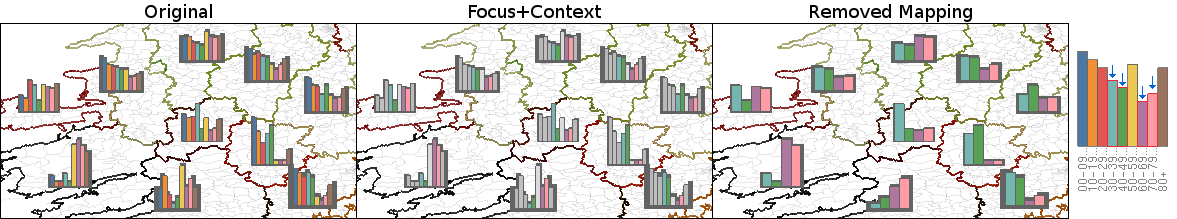
\includegraphics[width=1\textwidth]{images/f+cv2} %\vspace{-0.3cm}
\caption{Filtering options. The left shows the original image. The center shows focus+context rendering, which renders the context in greyscale. The right image shows a multivariate glyph mapping filter, which re-renders the data based on the focus dimensions. The legend indicates the focus dimensions using the blue arrows. Refer to Section \ref{sec:filter}. The Munster area refers to the bottom-left glyph, which is notable for Case Study 3, Section \ref{sec:case03}.} \label{fig:f+c}  \vspace{-0.2cm}
\end{figure*}
\subsection{Smooth Merging and Splitting Transitions} \label{sec:transitions}
In order to increase the smoothness of user interaction and changes to glyph size when zooming or manipulating $m$, we apply smooth transitions to child glyph merging and parent glyph splitting. When the user reduces the number of glyphs by either zooming out of the map or increasing the level of detail, glyphs translate towards the origin of their parent in the hierarchy while the opacity is reduced until it is no longer visible. The parent increases in opacity until it is fully opaque, creating a smooth transition. When adding new glyphs (zooming in or reducing minimum scale), the new child glyphs translate away from their parent and increase in opacity to provide a similar effect. Using this technique, we fulfill the requirement for \textbf{T6 -- Fluid Interaction}. See Figure \ref{fig:transitions}. This dynamic animation is best viewed in the accompanying video (Section \ref{sec:video}).


\subsection{Dynamic Average Glyph Legend} \label{sec:legend}
We provide a dynamic average glyph legend to present how the multivariate data dimensions of the glyph are encoded. The advantage this provides is that each individual glyph on the map can be compared to the average shown in the legend. Each variate is given a label, which provides context to the user about what is presented. The data used to present the glyph is made meaningful by visualizing the average value of each dimension. In Figure \ref{fig:legend}, we can see that there seem to be some extreme values for the 80+ and 20--29 range, causing the average per area to be quite small overall.


\subsection{Attribute Filtering} \label{sec:filter}
Our first filter option is to re-calculate the glyph design with only the toggled dimensions. Each data dimension can be toggled using a check-box incorporated to represent data variates in the glyph design. This allows the user to focus on or emphasize data dimensions that may reveal trends. We support user filtering using focus+context rendering. We provide a gray-scale option which removes the color from context data dimensions, enabling easier comparison. This supports the requirements we outlined in \textbf{T5 -- Filtering}. See Figure \ref{fig:f+c}.

\subsection{Unit Area Density Indicators} \label{sec:indicate}
We present unit area density indicators that provide a visual queue indicating how hidden unit areas are distributed and encourage the user to explore the visualization through multiple levels of detail. When two child glyphs merge to form a parent, the child glyphs are then hidden. Our glyph design maps the number of merges to a range of different visual indicators that generally surround the glyph. See Table \ref{tab:glyph}. We offer four options:\\
\textbf{Outline:~} Outline maps the unit area quantity around each glyph to thickness. The thickness of the outline grows as more areas fall underneath a glyph.\\
\textbf{Size:~} Rather than provide an outline, the glyph's overall size increases as the glyph represents more unit areas. This works especially well with pie charts, that emulate a proportional map. \\
\textbf{Size+Outline:~} Size + Outline uses a combination of the two previous options.\\
\textbf{Shadows:~} Rather than an outline with a constant opacity, we enable the user to choose a gradient, enabling less occlusion in the representation.\\
These unit area density indicators are inspired by the work of Chung et al.\ \cite{chung2015glyph} where the indicator was effective but used to represent another data dimension (as opposed to the density of a map).
We also give the user an option to represent the indicator mapped to color. The color represents the scale the glyph encodes, as opposed to other visible encodings. This enables the user to gain an understanding of how manipulation of glyph density can affect the map if a transition is made. See Figure \ref{tab:glyph}. This addresses our requirements of \textbf{T4 -- Level-of-detail}.

\begin{figure}[t]
\centering
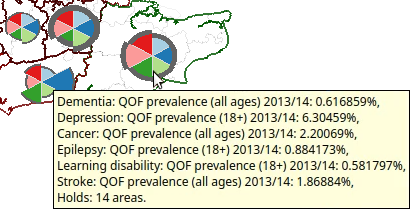
\includegraphics[width=0.5\linewidth]{images/ch5/onMouseOver} \vspace{-0.5cm}
\caption{By hovering over a glyph (for this example we use the south-east of England), the user is provided with details on demand of the multi-variate datavalues depicted and the number of areas represented by the glyph.} \label{fig:dod}
\end{figure}

\subsection{Interactive User Options} \label{sec:options}
We provide additional user options to support \textbf{T5 -- Filtering}. We present a range of user options including value range filters, advanced focus+context rendering options, estimated glyph placement, and context administrative areas.\\
\textbf{Data Range Options:} We provide data range filtering to enable customized local and global design options for dimension encoding. On a local range, the user can shift the value range to present the data dimensions based on the values found in the leaf nodes (the original dataset), or clamp the ranges amongst those that are currently being rendered to enable a more accurate data range to compare data dimensions. We also support global range options by enabling the user to depict each variant based on its range, or by creating a range based on the highest and lowest value of all mapped dimensions.  \\
\textbf{Advanced Filters:} We include two advanced filters to render focus+context for the user. For numerical values, the user can present focus+context based on values higher or lower than the average value per data dimension.\\
\textbf{Color Map:} We provide the user with a variety of color maps, selected from published research, including ColorBrewer \cite{brewer2003transition} (Refer to Table \ref{tab:glyph}) and Colorgorical \cite{gramazio2017colorgorical} (Refer to Figure \ref{fig:f+c}).\\
\textbf{Glyph Scaling:} We allow the user to scale the current size of the glyph. This enables the user to explore a ratio between the minimum scale and size of glyphs that meets their own data.\\
\textbf{Naive estimated glyph placement:} Using the current size of the glyph, we can support the user to make an estimation of the minimum screen space necessary to remove occlusion with the use of a button. This makes it easier to obtain a starting point, in order to decide the design of the map they would like to use. This can also be linked to the glyph scaling to allow for automatic re-placement when scaling the glyph.\\
\textbf{Context Administrative Areas:} We can provide additional context behind the areas by rendering every leaf area in a context view, which is shown in Figure \ref{fig:f+c}.\\
\textbf{Details on demand:} We allow the user to obtain precise insight into the multivariate data by providing a textual representation of the values associated with a glyph by hovering over any glyph. We also include the number of areas depicted to give better context to the underlying data. See Figure \ref{fig:dod}.

\section{Evaluation} \label{sec:video}
We evaluate our glyph placement for multivariate maps in two ways. First, we provide three cases for the use of the multivariate maps with varying data sources. We then provide a comparative evaluation of our glyph placement strategy against a standard Cartesian grid-based glyph placement to evaluate its effectiveness and any advantages or potential drawbacks against pre-existing techniques. We include a video representation of the case studies discussed in the paper. This can be found at the following link: \url{https://vimeo.com/314225790}.

\subsection{Case Studies}  \label{sec:case}
In order to evaluate our glyph placement strategy, we incorporate three case studies. In our first case study, we examine health indicators coupled with CCGs (Clinical Commissioning Groups) within England. Secondly, we examine the average income of US counties over 10 year periods. Finally, we look at the age distribution across the electoral divisions of the Republic of Ireland.


\textbf{Case 1: England's Clinical Commissioning Groups (CCGs): } \label{sec:case01}
Our first case uses a dataset focused on England's Clinical Commissioning Groups, which represent areas of NHS practices. People who reside in the area are generally expected to use the same practices. We explore the prevalence of afflictions per CCG area, including Dementia, Depression, Cancer, Epilepsy, Learning Disabilities, and Stroke. Refer to Figure \ref{fig:ccgs} to show an example of the CCGs represented \cite{publicHealthEngland}. There are over 200 CCGs. Figure \ref{fig:ccgs} also compares a naive glyph placement using region centroids with our glyph placement strategy. Placing glyphs in ever area centroid is one of the most common placement strategies.

For this example, overlapping glyphs are prevalent around London, Liverpool, and Manchester, if we simply render a glyph at each centroid (Figure \ref{fig:ccgs}, left). We start with the pie chart glyphs to obtain an overview of the data (\textbf{T1 -- occlusion}). As pie charts always extend to the maximum radius, combining our level-of-detail glyph placement algorithm combined with the estimated minimum size placement removes most of the occlusion, enabling visual comparison between the points (\textbf{T2 -- multivariate maps}, \textbf{T3 -- glyph placement}). The first trend we notice is that depression has a majority prevalence across most CCGs, although we can observe that the Kernow CCG  exhibits an uncommon distribution, caused by a larger distribution of cancer as opposed to other pie glyphs (Figure \ref{fig:ccgs}). At this point, we can filter out depression prevalence, however, we can glean a bit more information by switching glyph design. If we transition to the star-glyph, we can see that this is due to both the larger prevalence of cancer and low rate of depression in comparison to other prevalence values for CCGs (Figure \ref{fig:grid}(a)).
As the star glyphs have varying extents, we can reduce $m$ down to 0.8\% to increase the level of detail with no occlusion (\textbf{T4 -- level-of-detail}). At this scale, London is split into 3 zones, where we can see the northwest point has lower prevalence overall (Figure \ref{fig:case01}). We can investigate this by zooming in to London (\textbf{T6 -- smooth interaction}). We zoom in to see a larger number of areas (rendered by $m$). Not only do we find Barnet, Enfield, Hillingdon, and Hounslow to have low prevalence rates overall, but Bromley and Croydon in south London also show these signs (dementia, stroke, and cancer prevalence in particular). See Figure \ref{fig:case01}.

\begin{figure}[t]
,\subfloat{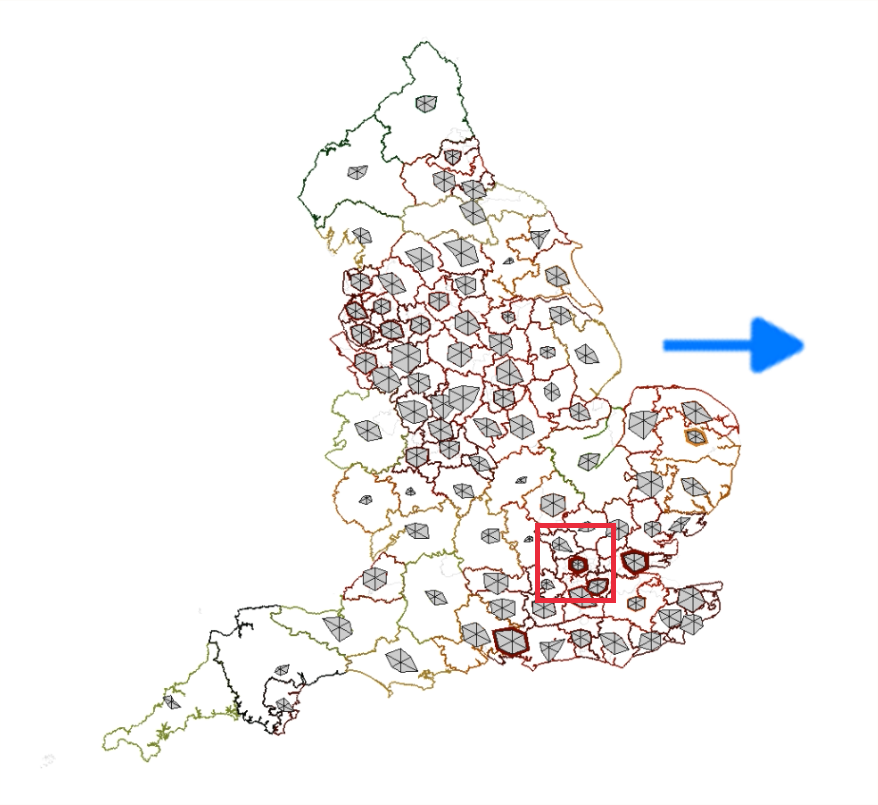
\includegraphics[width=0.48\linewidth]{images/ch5/london01}}
\subfloat{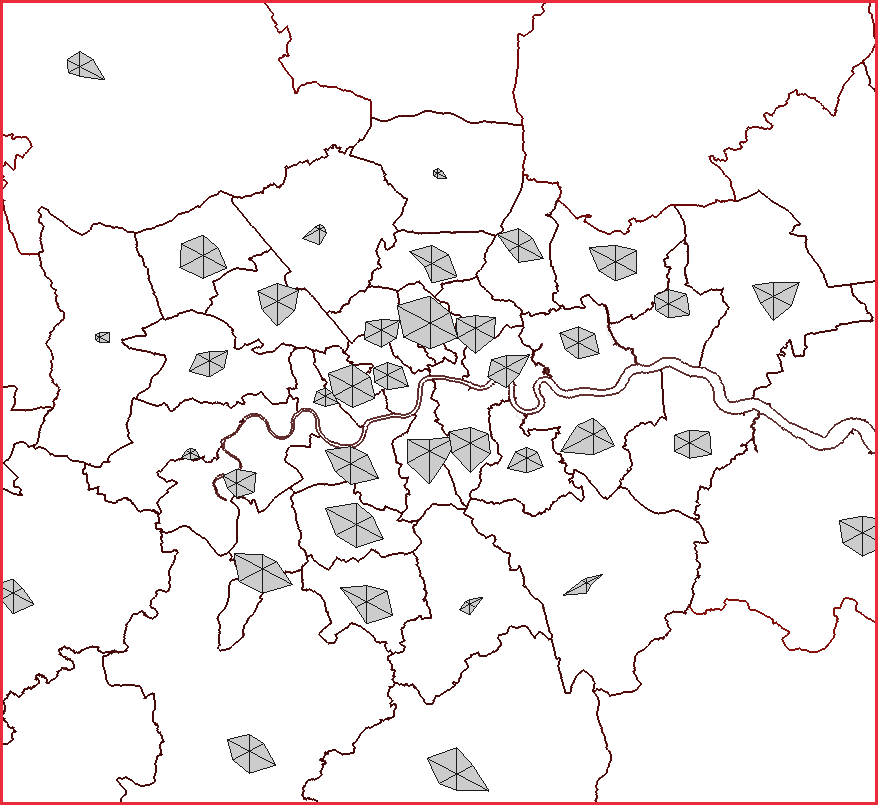
\includegraphics[width=0.48\linewidth]{images/ch5/london02-1}}
\caption{After identifying the southwest of London as having lower prevalence rates than the rest of London (red box), we zoom in to see the cause. We can see low prevalence rates are more frequent among the northwest, with some low prevalence rate in the southeast. We can also now identify the particular CCGs. Glyph scale increased for zoomed in view. See Section \ref{sec:case01}.} \label{fig:case01}
\end{figure}


\textbf{Case 2: Counties of the United States: } \label{sec:case02} 
Our second example explores counties in the US. We look at the average income over 40 years for each county in the United States from 1979, 1989, 1999, to 2009 in 10-year increments \cite{usCounties}. The US consists of over 3,000 counties.

Rendering the glyphs presents a large frequency of occlusion and therefore we use the estimated minimum size, $m$, to reduce the large number of glyphs to something more accessible.  Starting with the pie chart shows a standard distribution where the average income increases per time period (\textbf{T1 -- overview}). Since each glyph represents many areas, we adjust the range indicator to represent areas that are rendered, and switch to a polar area chart to visualize the data (Figure \ref{fig:grid}(b)). The wheel glyph shows higher income on the east and west coasts, with the lowest value glyphs across the center of the United States. Wyoming and Montana have some uncommon behavior, where 1979 and 2009 show a much stronger average income than their other variants. Zooming in, Wyoming exhibits a tendency to exhibit a higher average income in 1979 over the 40 years, independent of their standing amongst the rest of the US counties. The counties of Sublette and Teton are the exceptions to this which hold stronger mean incomes in 1999 and 2009. See Figure \ref{fig:case02}.

\textbf{Case 3: Electoral Divisions of the Republic of Ireland: } \label{sec:case03}
For our final case, we look at the electoral divisions of the Republic of Ireland. Our data set records population distribution across each division, which is split into nine groups, 0--9 years old, 10--19, 20--29...up to 80+ \cite{electoralDivisions}. There are over 3,400 electoral divisions in the Republic of Ireland.

Similar to Case 2, there are a large number of electoral divisions so we immediately choose to reduce the visible areas to a perceivable number using the estimated scale glyph placement, and adjust a filter to represent a clamped range. In this example, we use bar charts to represent the data. If we look towards Munster, we can see an unusual population distribution, where the proportion of the population, 50 or above, is uncommonly high, and the proportion of people, under 50, is uncommonly low (Figure \ref{fig:f+c}). Zooming in, Glanmore, Canuig, Tahilla, Derriana, Dawros, Ardea, Castlecove, and Caher seem to be the leading factors in this trend. See Figure \ref{fig:case03}.


\begin{figure}[t]
\subfloat{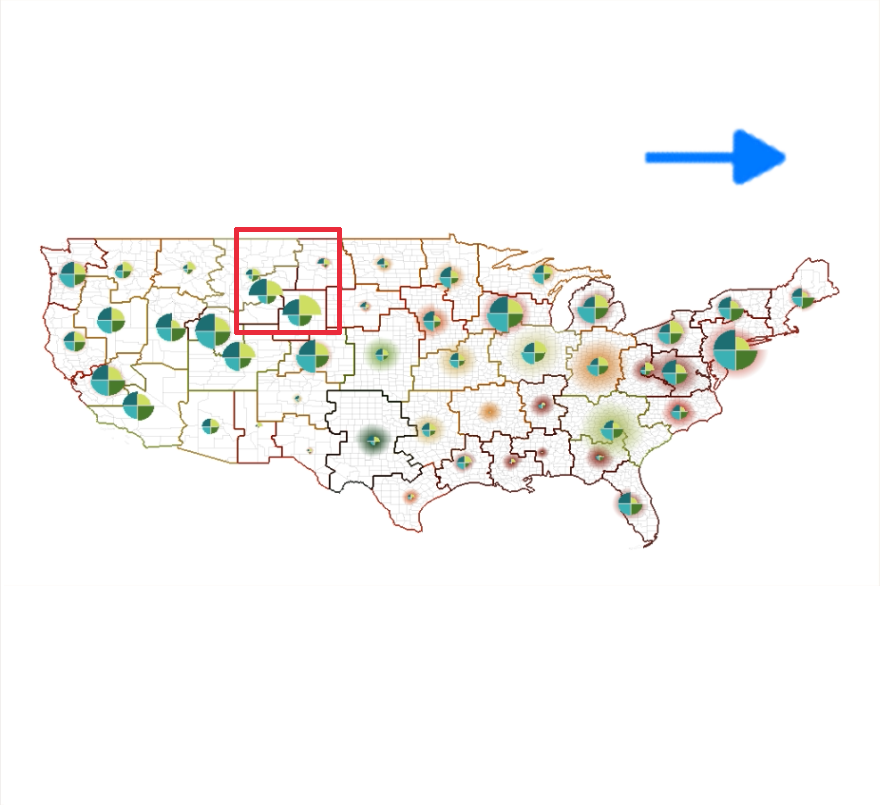
\includegraphics[width=0.48\linewidth]{images/ch5/us01}}
\subfloat{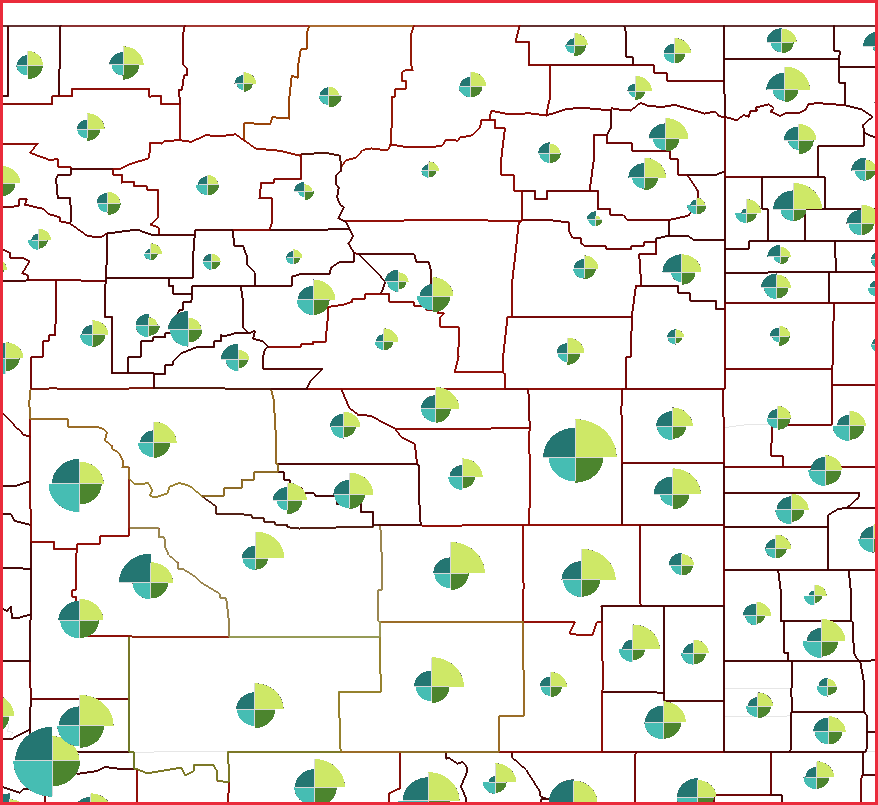
\includegraphics[width=0.48\linewidth]{images/ch5/us02-1}}
\caption{We notice counties around Wyoming and Montana have are higher average income in 1979 and 20019 than usual, We zoom in, and can verify this amongst particular counties. Glyph scale increased for zoomed in view. See Section \ref{sec:case02}.} \label{fig:case02}
\end{figure}
\begin{figure}[t]
\subfloat{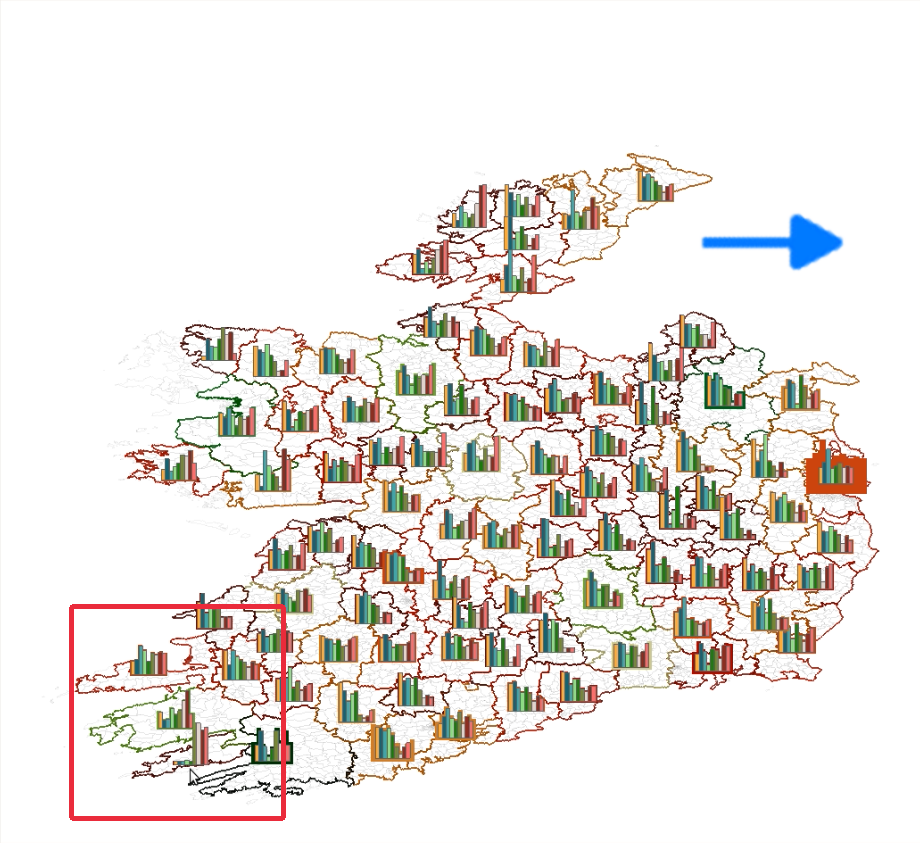
\includegraphics[width=0.48\linewidth]{images/ch5/ireland01}}
\subfloat{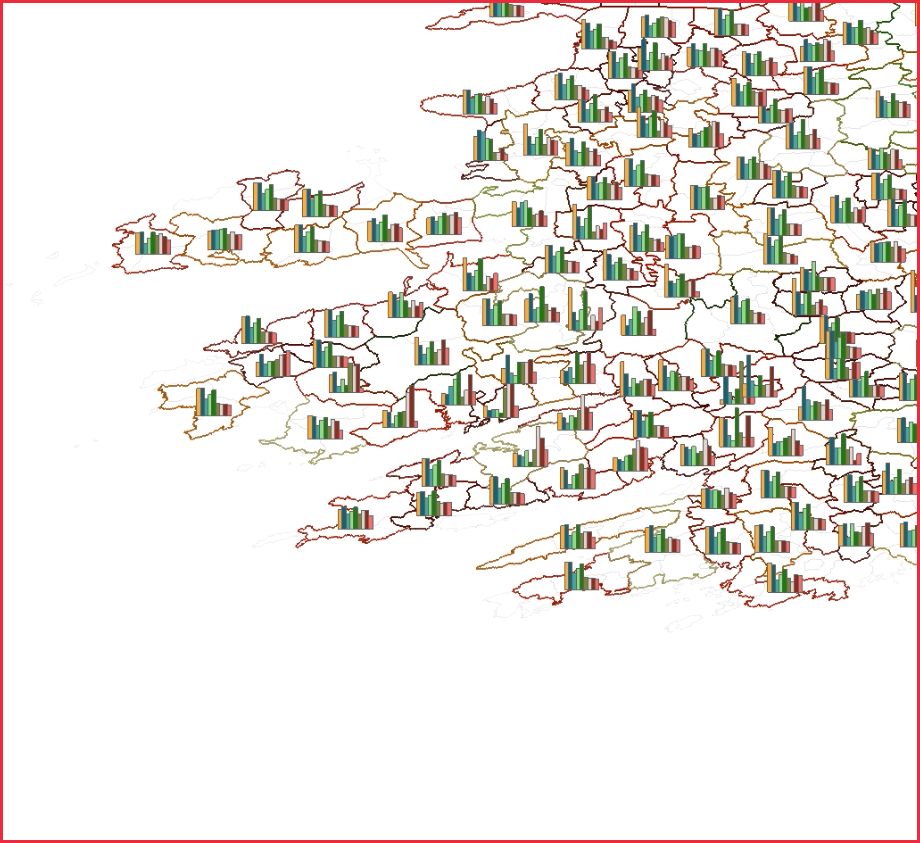
\includegraphics[width=0.48\linewidth]{images/ch5/ireland02}}
\caption{After noticing a strange inconsistency in the south-east of the Republic of Ireland, we zoom in and can verify that this trend can be found amongst a selection electoral divisions. Glyph scale increased for zoomed in view. See Section \ref{sec:case03}.} \label{fig:case03}
\end{figure}


\subsection{Comparative Evaluation: Grid-Placement vs. Dynamic Placement} \label{sec:grid}
We compare our implementation to a standard grid placement technique, in order to compare the advantages and disadvantages that can be found for both. We can also compare some of the problems that were brought up in our motivation section (Section \ref{sec:introMM}) to diagnose the effectiveness of the technique against some of these challenges.

We evaluate user interpretation of the data against a typical grid structure for glyph placement. We use a Cartesian grid (20$^2$) structure that places glyphs at approximately the same size and resolution as the algorithm developed in this paper. Each area is assigned to a cell of the grid, closest to its centroid, where glyphs are derived using the same process as our algorithm. In terms of design, we try to keep both structures similar. In our algorithm, we use a thickened outline to signify the unified area the glyph presents which is not possible for the grid placement version because unit areas are arbitrarily split using a Cartesian grid. We, therefore, show the presented areas using a lower line width to avoid over-representation. Other than this, all design elements are the same and we allow the user to adopt filters and user options identically. However, we use a standard grid structure and therefore the grid structure does not necessarily handle multiple levels of detail. Examples are shown in Figure \ref{fig:grid}.

\begin{sidewaysfigure*}[p] \centering
\subfloat{
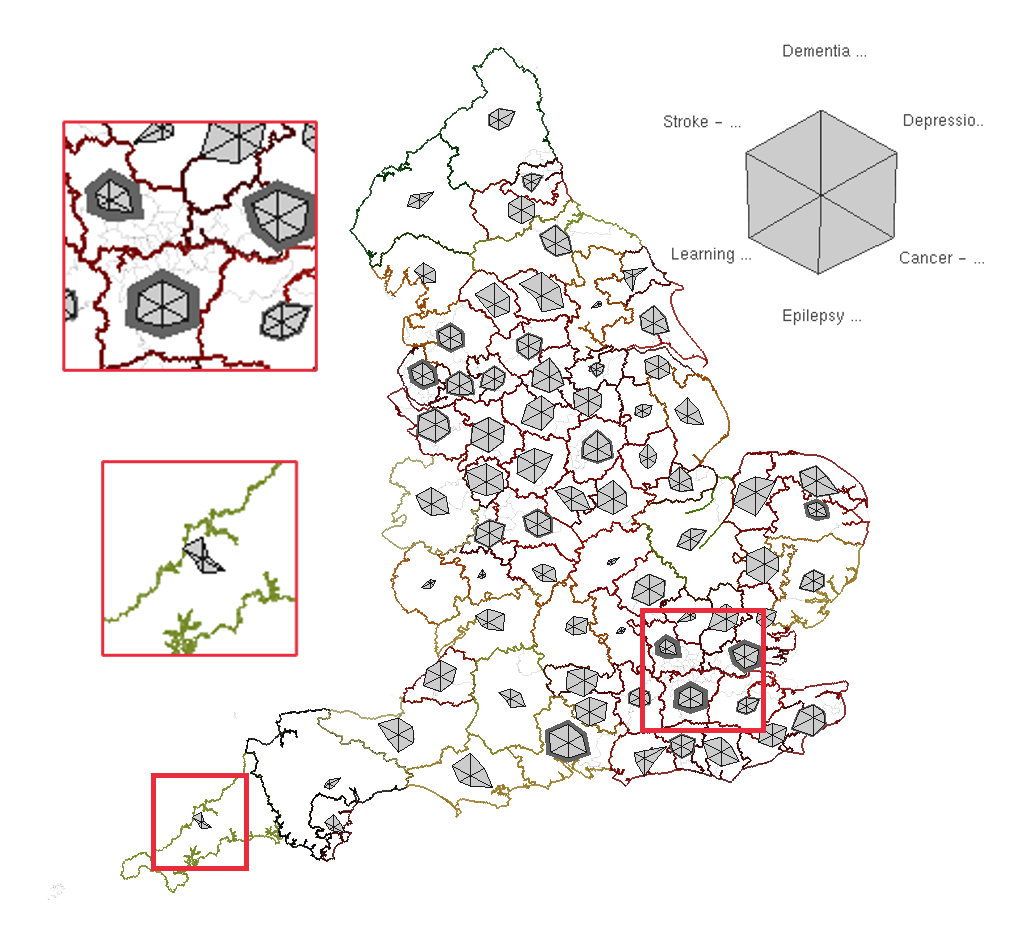
\includegraphics[width=0.32\textwidth]{images/ch5/CCGgridAFull2.png}}
\subfloat{
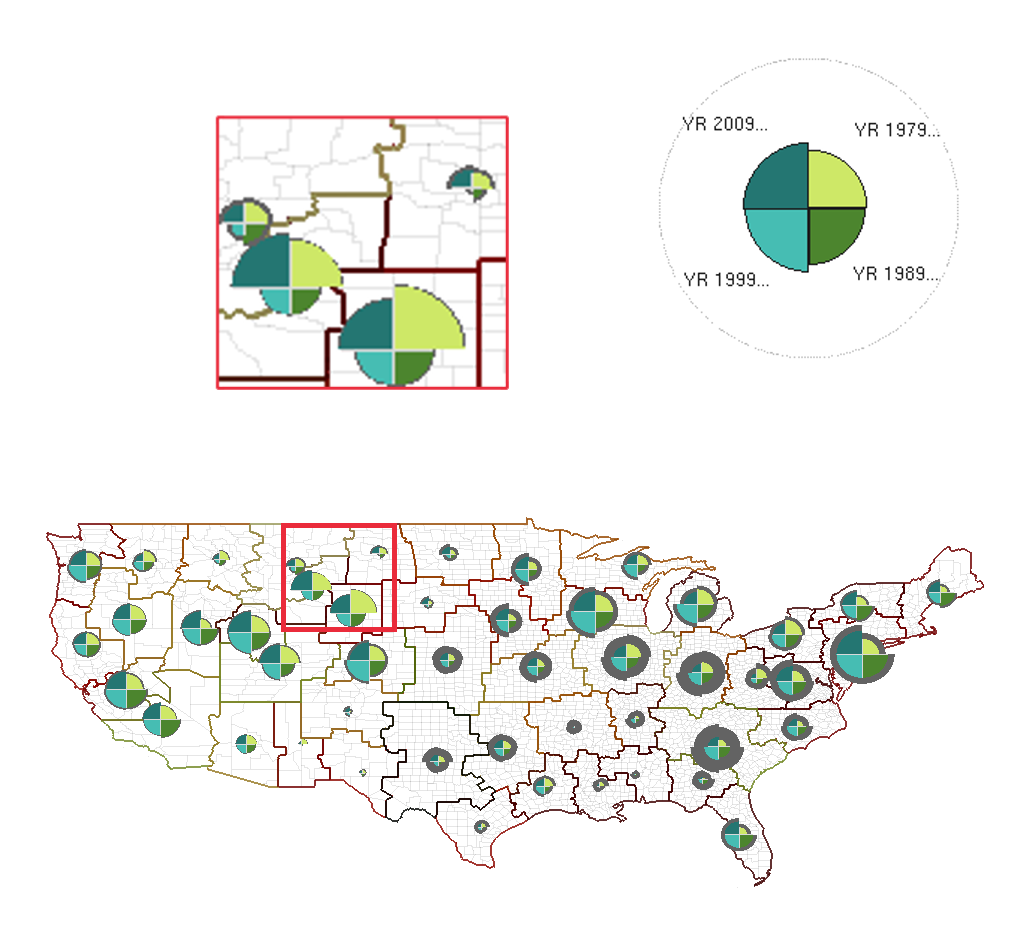
\includegraphics[width=0.32\textwidth]{images/ch5/USgridAFull2.png}}
\subfloat{
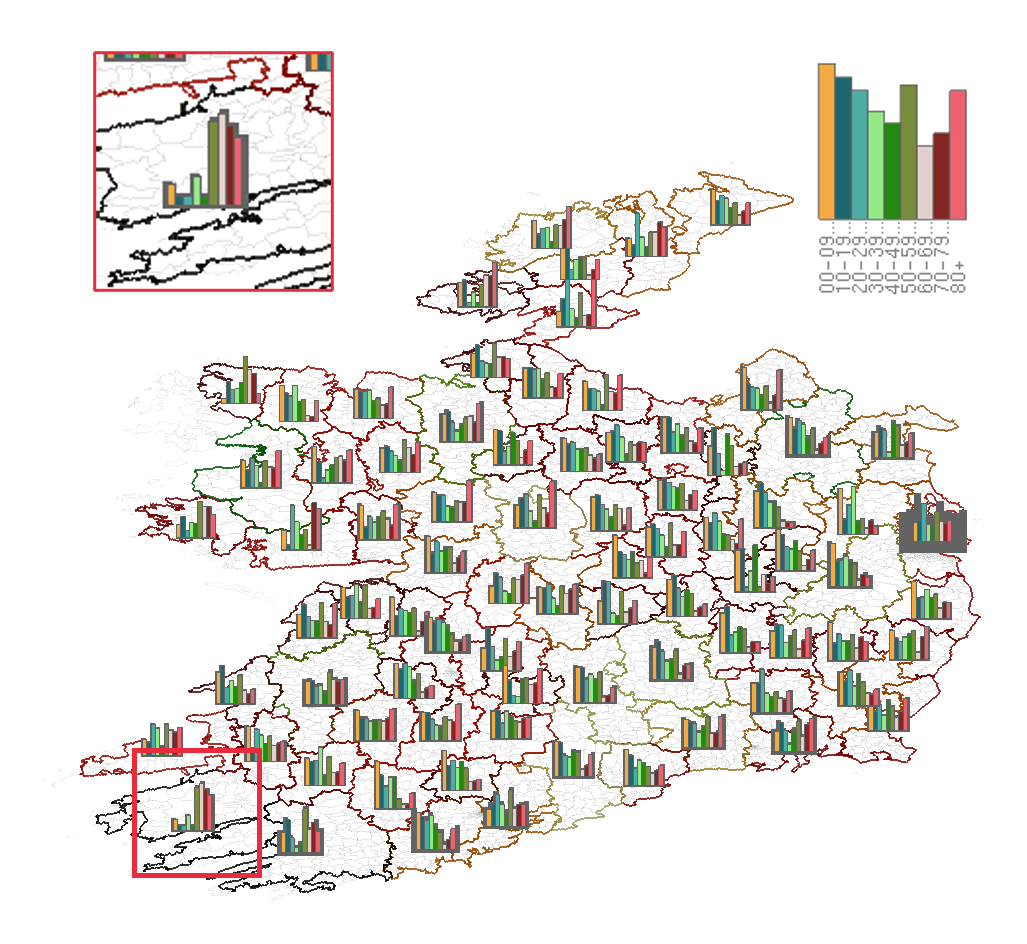
\includegraphics[width=0.32\textwidth]{images/ch5/irelandgridAFull2.png}}
\setcounter{subfigure}{0}
\subfloat[]{
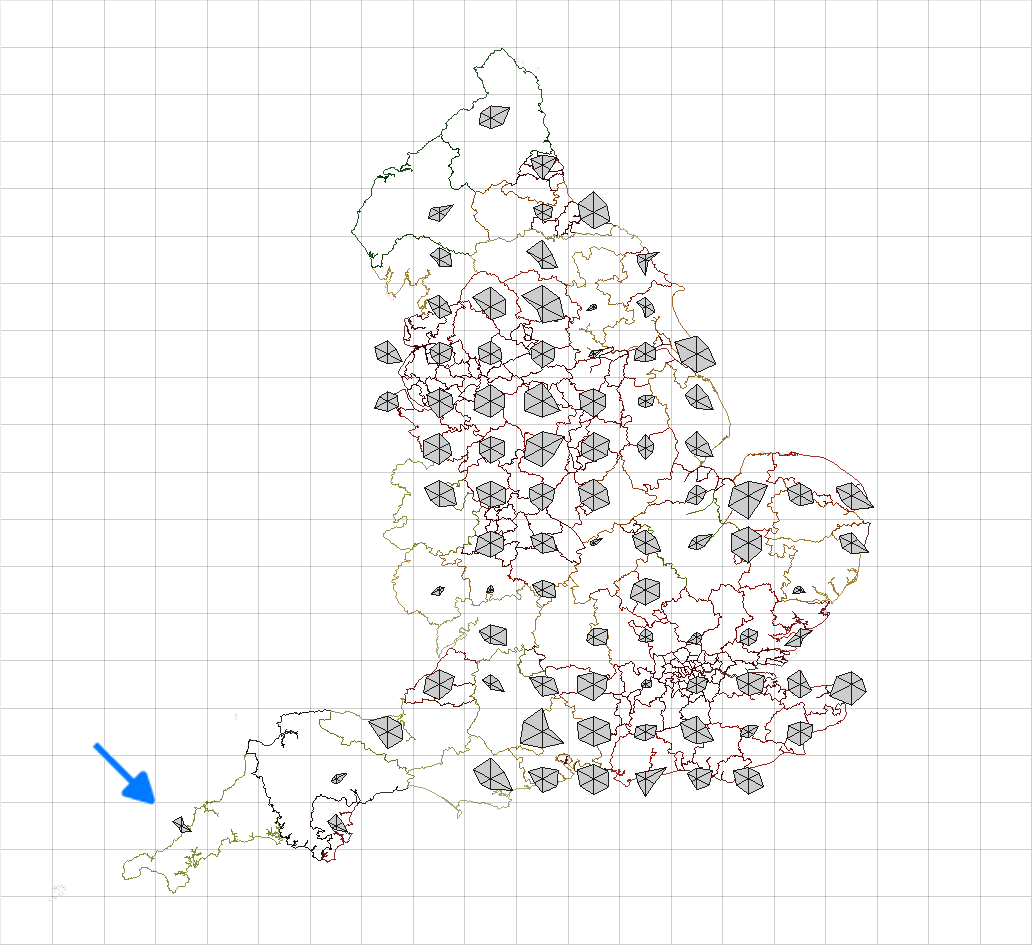
\includegraphics[width=0.32\textwidth]{images/ch5/CCGgridBFullAZ.png}}
\subfloat[]{
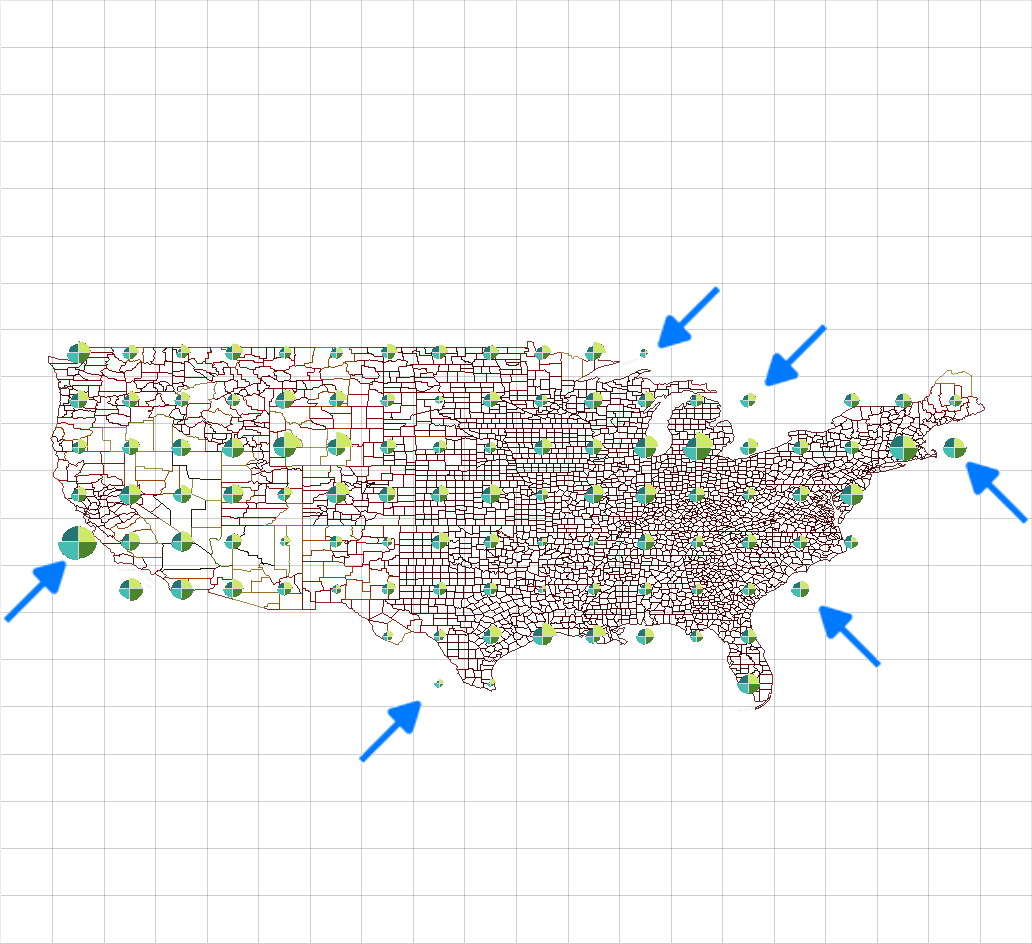
\includegraphics[width=0.32\textwidth]{images/ch5/USgridBFullAZ.png}}
\subfloat[]{
\includegraphics[width=0.32\textwidth]{images/ch5/irelandgridBFullAZ}}
\caption{Glyph-placement comparison: top row -- our method, bottom row -- grid-based. (a) Comparison of CCGs (b) Comparison of US Counties (c) Comparison of Ireland's Electoral Divisions. Glyphs based on grid-placement are often de-coupled from the geo-space the represent. The blue arrow signifies the cause of the incomparable data values. See Section \ref{sec:grid}.
} \label{fig:compare} \label{fig:grid}
\end{sidewaysfigure*}

We look at two main aspects of placement, geometric coupling, and value representation. First, we examine geometric coupling. As the grid is uniform, in all instances, the grid allows for a larger number of glyphs, however, this can be seen as a clear positive. If we start with Figure \ref{fig:grid}(a), it is sometimes difficult to verify where a glyph is when areas reside within a corner of multiple grid slots. If we look at the central-east coast of England, identifying even large areas becomes difficult. This is because the areas are considered uniform, and therefore are distributed uniformly, as opposes to our presented algorithm which attempts to avoid this as much as possible.  In example Figure \ref{fig:grid}(b), our placement uses fewer glyphs due to the large variance in wheel glyph extents, as opposed to the grid placement that presents roughly twice as many. The grid results in the same limitation as above, with strong difficulty in understanding how values are mapped to their glyph counterparts. We run into a second problem with the density of the areas, where administrative areas make it difficult to perceive where a grid cell covers, providing little understanding of the context. Both of these problems follow on to Figure \ref{fig:grid}(c).

For value representation, the algorithms do show differences, which is to be expected, in accordance with the modifiable areal unit problem \cite{openshaw1984modifiable}. For Figure \ref{fig:grid}(a), both representations pointed to the same observation in our case study. Figure \ref{fig:grid}(b), exhibits a significant difference. The grid-placement greatly skews the value representation of the US counties, due to some grid elements covering secluded cells. The west coast contains a grid cell with San Francisco, which causes most of the other glyphs to be quite small, independent of the data range option selected. It becomes difficult to compare the two placement options. Although that is the case, both placement schemes lead to the observation found that the time period of 1979 maps to a larger segment in Wyoming. Figure \ref{fig:grid}(c) also presents the observations found in our case study, although the concentration is more spread out, which can be considered better for examinations. If we consider the ability to zoom, we feel that only the Cartesian grid representation of the Republic of Ireland can lead to a fair comparison for observation, and this is only based on trial-and-error.


%\section{Future Work}
%There are many avenues for future work we can consider. At the moment, we use the raw derived centroid as a placement strategy. although this removes a lot of density and occlusion, there is still some wasted space. We believe that by adding some overlap removal, we could use space more efficiently, whilst still avoiding any decoupling problems. Although we present some case studies, the algorithm could be more carefully compared to other glyph placement strategies with a user-study evaluation. Although we think the use of transitions was a great tool for understanding variation, it is not always necessary. We feel that there are many avenues for exploring at multiple levels of detail. For example, directly zooming to a glyphs unit area's extents may not need to represent zooming, to speed up the exploration.
%\section{Conclusion}
%We present a glyph placement algorithm supporting multivariate geospatial visualization at different levels of detail.  We discuss how we create scale aware map, and apply the process to glyph placement. We also discuss the different glyph options and filters we have designed to support the exploration of multivariate data. Finally, we review the algorithm by examining the separate use cases and compare against a pre-existing glyph placement strategy.
%\begin{figure}[t]
%\centering
%\subfigure[]{
%\includegraphics[width=0.6\linewidth]{images/GlyphLegendAndFilter.png}}
%\caption{.} \label{fig:uahindicator}
%\end{figure}

\section{Conclusion}
With big data rapidly becoming ubiquitous within the field, many have been wondering what they must do to represent all the data given to them. At the EuroVis conference 2017, in his capstone presentation, Helwig Hauser brings up the idea of human vision bandwidth and discusses the brain's capability to interpret information. Hauser states that color and transparency are only temporary solutions and may not be useful when our data sets are 10 orders of magnitude larger than current data sets \cite{hauser2019from}. We consider this while looking at Schneiderman's information-seeking mantra, \emph{" Overview first, zoom and filter, then details-on-demand"}, specifically the first step, gaining an overview of the entire collection \cite{shneiderman1996eyes}. If we can no longer rely on color, how can we enable a full overview in one image? The answer may be simpler than expected, and that is to reduce the resolution of data to present.

Wong has already begun work on the topic of multi-resolution data \cite{wong1997adaptive}, however, his work emphasizes scientific visualization. We suggest \textit{low fidelity} visualization. Low-fidelity visualization describes a representation of visualization with a high level of abstraction. We believe that this can be used to present an overview of the data while (a) still presenting an authentic view of the underlying data (b) conveying close approximations of the underlying data, and (c) still allowing the user to clearly understand where and how zooming and filtering will be useful. However, implementing a low-fidelity view can be interpreted negatively. By creating approximations of data, value error may be introduced, and when values are associated with error the observer may be subject to false insight and false results. This issue is a well-known problem even outside of the visualization landscape. The Modifiable Areal Unit Problem (MAUP) considers how aggregating values confined to a 2D space can vastly change the results depending on which areas are grouped \cite{openshaw1984modifiable}.
We also consider that many people assume that something unseen, has been left unseen intentionally.

We believe that a low-fidelity visualization is a viable approach that can improve any visualization tool and new techniques can be used such as clutter reduction for visualization that would otherwise find difficulty with common reduction techniques.  We explore why low-resolution visualization should not be considered a barrier, and preferably a useful tool to avoid cognitive overload. We also discuss common negative sentiment and ways to address challenges that may be coupled with the idea.

\subsection{Hidden Data}
It is important to consider that there are many cases where data you visualize has already been transformed to reduce complexity. If we look at census data, by law, before any data is made public, the data needs to be both anonymized and grouped in order to protect the identity of persons both in name and location. %Expand
%\subsection{Background}

\subsection{Visual Perception}
Perception is a large research area within visualization and is a leading consideration when designing software and visualization techniques. This large amount of work can be broken down into discrete categories such as color \cite{lee2013perceptually,heer2012color,szafir2018modeling}, size \cite{mcnabb2018when,borgo2014order,gramazio2014relation}, and motion \cite{simons2000current, driver1992motion, huber2005visualizing}. However, research on this topic can vary widely to consider the work comparing ease of perception against other techniques in the form of user studies \cite{rittschof1998learning} or guidelines on perceivability within specific topics \cite{kong2010perceptual}. When considering a visualization technique, recognizing perceivabilty as a key challenge can transform your software into a critical analysis tool. 

Visual perception is more than just an understanding of digital phenomenon. Physical constraints can also play an important role in how techniques evolve. Pixel density is an important consideration when depicting data. In Chapter \ref{chap:userStudy}, we depict that when an area becomes smaller than 10 pixels, the error becomes prevalent when identifying the color, and performance time also increases. This has lead to many advances in space-filling algorithms, however, what happens when a space-filling algorithm is forced to present some data marks within a small pixel threshold. %Pixel Density

\subsection{Overview without full detail}
Let's reconsider the information-seeking mantra once more. An overview is considered the first step to understanding, and because of this, it is easy to consider this as everything that needs to be represented. However, this is not the case. If everything could be understood from an overview, there would be no need for a user to zoom in or filter in the first place. If we compare the overview of a visualization to a modern shop, we must consider the overview as our initial view of a shop. If we conclude the outside of the shop is the overview, then our main point of emphasis is that which is displayed in the at the entrance or on display in the window. If we consider the interior, we are likely to see signs which lead us to where we would like to go. An overview should be considered a gateway to enable zooming and filtering.

In order to make sure that reducing the resolution does not affect exploration, we can use techniques to minimize the effects of aggregation. In this section, we discuss two key areas: resolution indication and uncertainty visualization.
\begin{table}[b]
\includegraphics[width=0.7\linewidth]{images/ch7/visualchannels}
\caption{Visual channels presented by Borgo et al.\ \cite{borgo2013glyph}. Refer to Section \ref{sec:reso}} \label{tbl:visualchannels}
\end{table}
\subsubsection*{Resolution Indication} \label{sec:reso}
If area resolution varies across 2D space, it is important to visualize where resolution may lie. We can use visual design variables in order to depict the spatial frequency of data. Borgo et al.\ combine multiple visual encoding variables to present a table of visual channels including geometric, optical, topological and relational, and semantic channels \cite{borgo2013glyph}. Refer to Table \ref{tbl:visualchannels}. In Section \ref{sec:indicate}, we present abstraction indicators by fixing the indicator to outline thickness, size or shadow. In this instance, hidden indicators are mapped to administrative area density. This makes the tool less useful for those already aware of the geospatial structure, however, this could be intrinsic for new users. %Add figure

\begin{figure}[t]
\includegraphics[width=0.4\textwidth]{images/ch7/trivariateH}
\caption{A depiction of a trivariate color map. The color map clearly expresses the distribution of values. By using this with low-fidelity visualization, we could depict what each area holds at multiple levels of detail. For example, a ratio of 3(oranges):2(apples):1(banana) would provide a better indication of how many values encapsulated by an area prefer orange rather than a less complex representation, leading to less confusion for the user (example highlighted in red).  Courtesy of McConchie \cite{mcconchie2018pop}} \label{fig:trivariate} %Extend
\end{figure}
\subsubsection*{Uncertainty Visualization}
Uncertainty visualization is a growing aspect of information visualization and applying these techniques to low-fidelity encapsulations is a logical process. Common uncertainty visualization normally uses visual mappings to convey error such as fuzzyness to detract careful analysis. However, when approaching uncertainty in low-resolution visualization, the idea sits in contrast with our attempt to coerce further analysis, causing fuzzyness to be a counter-intuitive mapping technique to use. We propose mitigating uncertainty by applying an advanced structure approach to your visual design of choice.
For example, categorical data could be mapped to present the majority, however, a second axis (saturation or opacity for example) can be used to present the percentage of the majority hold.
%If we use color as our visual channel to depict the most common attribute of `A',`B', and `C', we can apply a bivariate color map to propose a value at the intersection of the highest selection and second-highest selection.
We could increase this by modeling a tri-variate color map that depicts the weighting of objects between the three values, presented in Figure \ref{fig:trivariate}. 
There is also work on this technique for higher-dimensional data by Cheng et a \cite{cheng2019colormap}.  

\subsection{When to Consider Low Fidelity Visualization}
%The Objective
\begin{figure}[t]
\includegraphics[width=1\textwidth]{images/ch5/ccgsetPie2}
\caption{(left) The representation of population health data based on the Clinical Commisioning Groups (CCGs) of England \cite{publicHealthEngland}. Glyphs that are simply placed at the centroid of each region are over-plotted and occluded around London and Liverpool (indicated by blue arrows). (right) The result using level-of-detail scale-aware maps. Even at a small scale for the figure, we can still clearly differentiate each area's glyph.} \label{fig:occlusion}
\end{figure}

In order to use low fidelity visualization, we need to be able to identify when they are appropriate. We use Figure \ref{fig:occlusion} as our first example. \textbf{Occlusion} is likely the easiest criteria to spot. Our example plots glyphs to Clinical Commissioning Groups representing healthcare data. It is possible to reduce occlusion with other methods. For example, Dwyer et al.\ present the Fast Node Overlap Removal (FNOR) algorithm to avoid this \cite{dwyer2005fast}. However, this may not always be useful. In this case, we want to ensure that the glyphs are easily coupled to the geospatial context whilst the FNOR algorithm would remove this entirely in densely populated areas. In this case, areas are amalgamated to make both the glyphs and the underlying values perceivable.

Our second criteria is \textbf{data density}. Even if there is no occlusion, it is still possible for it to become difficult to perceive information. Space-filling techniques such as treemaps can avoid occlusion, but when you have to map millions of events, then the output can result in simple pixel representations of the data. Fekete and Plaisant present a paper working on a treemap for a million items represented \cite{fekete2002interactive}. We can see Figure \ref{fig:ch7treemap} makes it very difficult to see the granular data, which could hide some interesting information. 


\begin{figure}[t]
\includegraphics[width=0.7\textwidth]{images/ch7/treemap}
\caption{A treemap depicting a file system of over a million items. Color represents the file type. Image courtesy of Fekete and Plaisant \cite{dwyer2005fast}.} \label{fig:ch7treemap}
\end{figure}
%\section{Acknowledgments}
%We would like to thank KESS for contributing funding towards this endeavor. Knowledge Economy Skills Scholarships (KESS) is a pan-Wales higher level skills initiative led by Bangor University on behalf of the HE sector in Wales. It is partially funded by the Welsh Government's European Social Fund (ESF) convergence programme for West Wales and the Valleys. We would also like to thank XX and XX for help with proofreading the paper.

%-------------------------------------------------------------------------

%\bibliography{references}
%\clearpage
%%-------------------------------------------------------------------------
\begin{figure*} \centering
\includegraphics[width=1\textwidth]{images/ch5/CCGgridAFull.png}
\caption{Standard representation of the glyph placement algorithm using the CCGs of England \cite{publicHealthEngland}, with star glyphs. The glyph represents the prevalence of afflictions per CCG area. The legend represents the average prevalence across all glyphs. } \label{fig:sample1}
\end{figure*}
\begin{figure*} \centering
\includegraphics[width=1\textwidth]{images/ch5/CCGgridBFull.png}
\caption{A comparison piece for our CCG sample in Figure \ref{fig:sample1}. The grid-placement is a $20^2$ grid and assigns values in a similar fashion to our concept.}
\end{figure*}
\begin{figure*} \centering
\includegraphics[width=1\textwidth]{images/ch5/USgridAFull.png}
\caption{Standard representation of the glyph placement algorithm using counties of mainline United States. \cite{usCounties}, with polar area glyphs. The glyph represents the average income per household over four time periods, 1979, 1989, 1999, and 2009. The legend represents the average income across all glyphs. } \label{fig:sample2}
\end{figure*}
\begin{figure*} \centering
\includegraphics[width=1\textwidth]{images/ch5/USgridBFull2.png}
\caption{A comparison piece for our US counties sample in Figure \ref{fig:sample2}. The grid-placement is a $20^2$ grid and assigns values in a similar fashion to our concept.}
\end{figure*}
\begin{figure*} \centering
\includegraphics[width=1\textwidth]{images/ch5/irelandgridAFull.png}
\caption{Standard representation of the glyph placement algorithm using electoral divisions of the Republic of Ireland. \cite{electoralDivisions}, with bar glyphs. The glyph represents the age distribution per electoral division in 10 year increments up to 80. The legend represents the average age representation across all glyphs. } \label{fig:sample3}
\end{figure*}
\begin{figure*} \centering
\includegraphics[width=1\textwidth]{images/ch5/irelandgridBFull.png}
\caption{A comparison piece for our electoral divisions sample in Figure \ref{fig:sample3}. The grid-placement is a $20^2$ grid and assigns values in a similar fashion to our concept.}
\end{figure*}
%%\begin{figure*}
%%\centering
%%\subfloat{
%%\includegraphics[width=0.18\linewidth]{images/transition/01.png}}
%%\subfloat{
%%\includegraphics[width=0.18\linewidth]{images/transition/02.png}}
%%\subfloat{
%%\includegraphics[width=0.18\linewidth]{images/transition/03.png}}
%%\subfloat{
%%\includegraphics[width=0.18\linewidth]{images/transition/04.png}}
%%\subfloat{
%%\includegraphics[width=0.18\linewidth]{images/transition/05.png}}\\
%%\subfloat{\includegraphics[width=0.12\linewidth]{images/transition/11}}
%%\subfloat{\includegraphics[width=0.12\linewidth]{images/transition/12}}
%%\subfloat{\includegraphics[width=0.12\linewidth]{images/transition/13}}
%%\subfloat{\includegraphics[width=0.12\linewidth]{images/transition/14}}
%%\subfloat{\includegraphics[width=0.12\linewidth]{images/transition/15}}
%%\subfloat{\includegraphics[width=0.12\linewidth]{images/transition/16}}
%%\subfloat{\includegraphics[width=0.12\linewidth]{images/transition/17}}
%%\caption{An example of a smooth transition made between two child glyphs. Both child glyphs decrease in opacity, whilst the new parent glyph increases in opacity. Refer to Section \ref{sec:transitions}.} \label{fig:grid}
%%\end{figure*}
%%\begin{figure}[t]
%%\centering
%%\subfigure[]{
%%\includegraphics[width=0.08\textwidth]{images/outline0.png}}
%%\subfigure[]{
%%\includegraphics[width=0.08\textwidth]{images/outline1.png}}
%%\subfigure[]{
%%\includegraphics[width=0.08\textwidth]{images/outline2.png}}
%%\subfigure[]{
%%\includegraphics[width=0.08\textwidth]{images/outline3.png}}
%%\subfigure[]{
%%\includegraphics[width=0.08\textwidth]{images/outline4.png}}
%%\caption{ The different types of unit area quantity indicators. (a) No indicator. (b) Outline. (c) Size. (d) Size+Outline. (e) Shadow.} \label{fig:uahindicator}
%%\end{figure}
%%\begin{figure}[t]
%%\centering
%%\subfigure[]{
%%\includegraphics[width=0.08\textwidth]{images/pie.png}}~~~~
%%\subfigure[]{
%%\includegraphics[width=0.08\textwidth]{images/polarareachart.png}}~~~~
%%\subfigure[]{
%%\includegraphics[width=0.08\textwidth]{images/bar.png}}~~~~
%%\subfigure[]{
%%\includegraphics[width=0.05\textwidth]{images/star.png}}~~~~
%%\caption{(a) Pie Chart (b) Polar Area Chart (c) Bar Chart (d) Star Chart. Each glyph represents the same data attributes.} \label{fig:glyphs}
%%\end{figure}
%\begin{figure*}[b]
%\centering
%\subfigure[]{\includegraphics[width=0.48\linewidth]{images/belowAverageFilter.png}}
%\subfigure[]{\includegraphics[width=0.48\linewidth]{images/aboveAverageFilter.png}}
%\caption{(a) Below Average Query Filter. (b) Above Average Query Filter. Refer to Section \ref{sec:filter}.} \label{fig:advancedfilter}  \vspace{-0.2cm}
%\end{figure*}
%
%\begin{figure*}[b]
%\centering
%\subfloat{\includegraphics[width=0.48\linewidth]{images/leafPerDimension.png}}
%\subfloat{\includegraphics[width=0.48\linewidth]{images/clampedPerDimension.png}}\\
%\subfloat{\includegraphics[width=0.48\linewidth]{images/leafOverall.png}}
%\subfloat{\includegraphics[width=0.48\linewidth]{images/clampedOverall.png}}\\
%\caption{Data Range Options. Refer to Section \ref{sec:filter}.} \label{fig:clamp}  \vspace{-0.2cm}
%\end{figure*}



